\section{Introduction}

Model uncertainty is an essential part of mathematical modelling, but is particularly acute in mathematical finance and economics where one cannot base models on well-established physical laws. 
Until recently, these models were mostly conceived in a three-step fashion: 
1) gathering statistical properties of the underlying time-series or the so-called stylised facts;
2) handcrafting a parsimonious model, which would best capture the desired market characteristics without adding any needless complexity and 
3) calibration and validation of the handcrafted model.
Indeed, model complexity was undesirable, amongst other reasons, for increasing the computational effort required to perform calibration but, in particular, also pricing and risk calculations.
With greater uptake of machine learning methods and greater computational power, more complex models can now be used. 
This is due to the fact that arguably the most complicated and computationally expensive step of calibration has been addressed. 
Indeed, the seminal paper~\cite{Hernandez2016ModelNetworks} used neural networks to learn the calibration map from market data directly to model parameters. Subsequently, many papers followed \cite{Liu2019ACalibration,Ruf2020NeuralReview,Benth2020AccuracyCurves,Gambara2020ConsistentCalibration,Sardroudi-Khosrawi2019PolynomialCalibration,Horvath2020DeepModels,Bayer2019OnModels,Bayer2018DeepModels,Vidales2018UnbiasedPDEs}. 
However, these approaches focused on the calibration of a fixed parametric model but did not address perhaps even more important issues -- model selection and model uncertainty. 

The approach taken in this work is fundamentally different in the sense that we let the data dictate the model, however, we impose a strong prior on the model form.
This is achieved by using SDEs for the model dynamics, but instead of choosing a fixed parametrisation for the model SDEs, we allow the drift and diffusion to be given by overparametrised neural networks.
We will refer to these as neural SDEs.   
These are shown to not only provide a systematic framework for model selection but also, quite remarkably, to produce robust estimates of the derivative prices. 
Here, the calibration and model selection are done simultaneously. 
In this sense, model selection is data-driven. 
Since the neural SDE model is overparametrised, there is a large pool of possible models and the training algorithm selects a model. 
Unlike in handcrafted models, individual parameters do not carry any meaning. 
This makes it hard to argue why one model is better than another. 
Hence, the ability to efficiently compute interval estimators, which algorithms in this work provide, is critical.

\subsection{Brief overview of prior non-parametric methods}

Non-parametric calibration of SDE coefficients dates back to at least~\cite{Avellaneda1997CalibratingMinimization}, where the functional form of the volatility parameter was obtained by minimising a cost functional given by the Kullback-Leibler divergence and involves solving a high-dimensional system of parabolic PDEs. Similar to our approach, their algorithm can be used to interpolate between implied volatilities of traded options in an arbitrage-free way.

A more modern approach was considered in~\cite{Guo2017LocalTransport}, where time continuous martingale optimal transport was applied to interpolate between initial and final asset price distributions, to calibrate the local volatility function in a non-parametric way. 
A similar idea was considered in~\cite{Guo2022CalibrationTransport}, where semi-martingale optimal transport was used instead. 
The cost function given by the prices of European options was optimised to obtain the functional form of an LSV model. The resulting fully non-linear HJB equations stemming from the dual of the convex optimisation problem then had to be solved numerically. Following this, \cite{Guo2018PathDerivatives} consider calibration via semi-martingale optimal transport for path-dependent derivatives, such as barrier and lookback options, which accordingly translate to solving a path-dependent PDE.

In parallel to this work Cuchiero, Khosrawi, and Teichmann~\cite{Cuchiero2020AModels} considered local stochastic volatility models with the leverage function approximated with a neural network. Their model can be seen as an example of a neural SDE.

\subsection{Problem overview}\label{sec problem overview}

Let us now for a moment consider a filtered probability space~$(\Omega, \Ff, \FF,\PP)$, where ${\FF\defEqual \{\Ff_t\}_{t\in[0, T]}}$ and a random variable~$\Psi \in L^2(\Ff_T)$ that represents the discounted payoff of a derivative (typically illiquid and path-dependent). 
The problem of calculating a market-consistent price of a financial derivative can be seen as equivalent to finding a map that takes market data (e.g., prices of underlying assets, interest rates, prices of liquid options) and returns a no-arbitrage price of the derivative.
Typically an It\^{o} process~$\{X_t^\theta\}_{{t}\in[0, T]}$, with parameters~$\theta \in \RR^q$ has been the main component used in constructing such a pricing function. 
Such a parametric model induces a martingale probability measure, denoted by~$\QQ(\theta)$, which is then used to compute no-arbitrage prices of derivatives.

In our work, the market data (input data) is represented by payoffs~$\{\Phi_i\}_{i=1}^M$ of liquid derivatives, and their corresponding market prices~$\{\Pp(\Phi_i)\}_{i=1}^{M}$.
We will assume throughout that this price set is free of arbitrage. 
To make the model~$\QQ(\theta)$ consistent with market prices, one seeks parameters~$\theta^{*}$ such that 
the difference between~$\Pp(\Phi_i)$ and~$\EE^{\QQ(\theta^*)}[\Phi_i]$ is minimised for all~$i\in\{1,\ldots,M\}$ with respect to some metric.
If for all~$i\in\nobreak\{1,\ldots, M\}$  we have~$\Pp(\Phi_i) = \EE^{\QQ(\theta^*)}[\Phi_i]$, then we will say the model is consistent with the market data (perfectly calibrated).
%If the number of parameters~$p$ is greater than the number of inputs then, 
There may be infinitely many models that are consistent with the market.
This is called Knightian uncertainty~\cite{Watkins1922KnightsProfit, Cohen2018DataApproach}. 



Let~$\Mm$  be the set of all martingale measures/models that are perfectly calibrated to market inputs. 
In the robust finance paradigm~\cite{Hobson1998RobustOption, Cox2011RobustOptions}, one takes a conservative approach and instead of computing a single price (that corresponds to a model from~$\Mm$) one computes the price interval~$(\inf_{\QQ \in \Mm}\EE^{\QQ }[\Psi],\sup_{\QQ \in \Mm}\EE^{\QQ }[\Psi])$. The bounds can be computed using tools from martingale optimal transport, which also, through the dual representation, yield the corresponding super- and sub-hedging strategies, \cite{Beiglbock2013Model-independentApproach}. Without imposing further constraints, the class of all calibrated models~$\Mm$ might be too large and the corresponding bounds too wide to be of practical use \cite{Eckstein2019RobustNumerics}. There is, however, an effort to incorporate further market information to tighten the pricing interval \cite{Nadtochiy2017RobustSkew}. Another shortcoming of working with the entire class of calibrated models~$\Mm$ is that, in general, it is not clear how to obtain a practical/explicit model out of the measures that yield the price bounds. For example, such explicit models are useful when one wants consistently calibrate under a pricing measure~$\QQ$ and the real-world measure~$\PP$ as needed for risk estimation and stress testing \cite{Broadie2011EfficientSimulation, Pelsser2016TheModeling} or learn hedging strategies in the presence of transaction costs and illiquidity constrains \cite{Buehler2019DeepHedging}.

\subsection{Neural SDEs}\label{sec nsdes}

Fix~$T>0$ and for simplicity assume constant interest rate~$r\in \RR$. 
Consider a parameter space~$\Theta = \Theta^b\times \Theta^\sigma \subseteq \RR^{q}$ and parametric functions~${b:[0,T]\times\RR^d \times \Theta^b \rightarrow \RR^{d}}$ and~${\sigma:[0,T]\times\RR^d \times \Theta^\sigma \rightarrow \RR^{d \times n}}$. Let~$(\Omega, \Ff, \QQ)$ with~$\Omega = \Cc([0,T];\RR^n)$ be a probability space  equipped with the canonical filtration~$\FF\defEqual\{\Ff_t\}_{t\in[0,T]}$ of the~$n$-dimensional Brownian motion~$\{W_t\}_{t\in[0,T]}$. 
We consider the following parametric SDE
\begin{equation}\label{eq:nsde}
\D X^{\theta}_t= b\left(t,X_t^{\theta}; \theta\right) \D t + \sigma\left(t,X_t^\theta;\theta \right)\D W_t\,,\,\,\, X^\theta_0 = x_0\,,\,\,\, t \in [0,T]\,.
\end{equation}
 By imposing suitable conditions on the coefficients~$(b,\sigma)$, we know that the unique solution to~\eqref{eq:nsde} exists, \cite[Chapter 2]{Krylov1980ControlledProcesses}. 
These conditions can be satisfied by neural networks (Definition~\ref{def:neuralnet}), e.g. by using suitably regular activation functions and by applying weight clipping or by taking regular and uniformly bounded activation functions. Throughout the work, we assume that~\eqref{eq:nsde} has a unique strong solution.
We split~$X^\theta$, which is the entire stochastic model, into traded assets and non-tradable components. 
Let~$X^\theta=(S^\theta, V^\theta)$, where~$S$ are the traded assets and~$V$ are the components that are not traded. 
We will assume that for all~$t\in[0,T]$, $x=(s, v)\in\nobreak\RR^d$ and~$\theta \in \Theta$ that
%\[
%\begin{array}{rll}
%b(t, (s,v); \theta) &= 
%\begin{bmatrix}
%rs \\ b^V(t,(s,v);\theta)
%\end{bmatrix} &\in\RR^d \\[15pt]
%\sigma(t,(s,v);\theta) &= \begin{bmatrix}\sigma^S(t,(s,v);\theta) \\ \sigma^V(t,(s,v);\theta)\end{bmatrix} &\in\RR^{d\times n}\,.
%\end{array}
%\]
\begin{align*}
b(t, (s,v); \theta) &= 
\begin{bmatrix}
rs \\ b^V(t,(s,v);\theta)
\end{bmatrix}\in\RR^d \;\textup{ and }\;
\sigma(t,(s,v);\theta) &= \begin{bmatrix}\sigma^S(t,(s,v);\theta) \\ \sigma^V(t,(s,v);\theta)\end{bmatrix}\in\RR^{d\times n}\,.
\end{align*}
Then we can write~\eqref{eq:nsde} as
\begin{equation}\label{eq:nsde2}
\begin{split}
\D S^{\theta}_t & = r S_t^{\theta} \,\D t + \sigma^S(t,X_t^\theta;\theta )\,\D W_t\,,\\
\D V^\theta_t & = b^V(t,X_t^{\theta}; \theta) \,\D t + \sigma^V(t,X_t^\theta;\theta )\,\D W_t\,,\\
X^\theta_t & = \left(S^\theta_t, V^\theta_t\right)	\,.
\end{split}
\end{equation}
Observe that~$\sigma^S$ and~$\sigma^V$, set to take values in the space of appropriately shaped matrices, encode arbitrary correlation structures between the traded assets and the non-tradable components.
Moreover, we immediately see that~$\{\E^{-rt}S_t\}_{t\in[0, T]}$ is a (local) martingale and thus the model is free of arbitrage. 

In a situation when~$(b,\sigma)$ are defined to be neural networks from Definition~\ref{def:neuralnet}, we call the SDE~\eqref{eq:nsde} a neural SDE and we formally denote by~$\Mm^{\text{nsde}}(\theta)$ the class of all solutions to~\eqref{eq:nsde}. 
Heuristically speaking, due to the universal approximation property of neural networks (see Theorem~\ref{thm:UAT} or~\cite{Hornik1991ApproximationNetworks, Sontag1997CompleteNetworks, Cuchiero2019DeepODEs}), we can expect~$\Mm^{\text{nsde}}(\theta)$ to contain a large class of SDEs solutions.
Furthermore, neural networks can be efficiently trained with stochastic gradient descent methods and hence one can seek calibrated models in~$\Mm^{\text{nsde}}(\theta)$. 
Finally, neural SDE integrates black-box neural network-type models with known and well-studied SDE models. 
One consequence of that is that one can: a)~consistently calibrate these under the risk-neutral measure as well as the real-world measure; b)~easily integrate additional market information, e.g. constraints on realised variance; c)~verify martingale property. We want to remark that for simplicity we work in a Markovian setting, but one could consider neural SDEs with path-dependent coefficients and/or consider more general noise processes.

We will denote the law of~$X^{\theta}$ on~$\Cc([0,T];\RR^d)$ by
$$\QQ(\theta) \defEqual \Ll(\{X^\theta_t\}_{t\in[0,T]}) \defEqual \QQ \circ (X^\theta)^{-1}.$$ 
Consider a payoff function~${\phi:\Cc([0, T];\RR^d) \to \RR}$ for some path-dependent financial derivative. 
It is well known that the expectation under~$\QQ$ and under the push-forward measure~$\QQ \circ (X^\theta)^{-1} = \QQ(\theta)$ satisfy
\begin{align*}
\EE^{\QQ}\Big[\phi(X^\theta)\Big] &= \int_{\Cc([0,T];\RR^n)} \phi\left(X^\theta(\omega)\right)\,\QQ(\D\omega)  \\
&= \int_{\Cc([0,T];\RR^d)} \phi(\tilde \omega)\,\big(\QQ\,\circ\, (X^\theta)^{-1}\big)(\D\tilde \omega) \\
&= \EE^{\QQ(\theta)}[\phi(X)]\,.
\end{align*}
Thus, for~$\phi:\Cc([0,T];\RR^d) \to \RR$ we see that we can either work with~$\QQ$, with~$W$ as the canonical process and the random variable~$\Phi = \phi(X^\theta)\in L^2(\Ff_T, \QQ)$ or equivalently with~$\QQ(\theta)$,~$X^\theta$ as the canonical process and the random variable~${\phi(X) \in L^2(\Ff_T, \QQ(\theta))}$.
%In the rest of the work, we will be abusing notation by writing~$\Phi$ as both the payoff and the mapping~$\Cc([0, T];\RR^d) \to \RR$.
Later, we will also consider an empirical approximation of~$\QQ(\theta)$, based on~$N$ iid copies of~\eqref{eq:nsde}, which will be denoted by~$\QQ^N(\theta)$, i.e.,~$\QQ^N(\theta)\defEqual\frac{1}{N} \sum_{i=1}^N \delta_{X^{i, \theta}}$. See Section~\ref{sec learning hedging strategy} for more details.


Given a loss function~$\ell :\RR \times \RR \to \RR^{+}$, the search for a calibrated model can be written as 
\[
\theta^{\ast} \in \argmin_{\theta \in\Theta}\sum_{i=1}^M \ell\left(\EE^{\QQ(\theta)}[\Phi_i],\Pp(\Phi_i) \right)\,.
\] 
To consistently extend the calibration to the real-world measure, assume that the risk-neutral calibration described above has been completed and assume that we are given some statistical facts, e.g. moments or other distributional properties, that the price process (or the non-tradable components) should satisfy.

Let~${\zeta:[0, T]\times \RR^d \times \RR^q \to \RR^n}$ be another parametric function (e.g. a neural network). We extend the parameter space to~$\Theta = \Theta^b\times \Theta^\sigma \times \Theta^\zeta \subseteq \RR^{q}$
and let 
\[
\begin{split}
b^{S,\PP}(t,X^\theta_t;\theta) & \defEqual  r S^\theta_t + \sigma^S(t,X^\theta_t; \theta) \zeta(t,X^\theta_t;\theta)\,,\\
b^{V,\PP}(t,X^\theta_t;\theta) & \defEqual  b^V(t,X^\theta_t;\theta) + \sigma^V(t,X^\theta_t; \theta) \zeta(t,X^\theta_t; \theta)\,.
\end{split}
\]
We now define a real-world measure~$\PP(\theta)$ via the Radon--Nikodym derivative 
\[
\frac{\D\PP(\theta)}{\D\QQ(\theta)} \defEqual  \exp\left(-\int_0^T \zeta(t,X^\theta_t;\theta) \,\D W_t - \frac12 \int_0^T |\zeta(t,X^\theta_t;\theta)|^2\,\D t \right)\,.
\]
Under appropriate assumptions on~$\zeta$ (e.g. bounded) the measure~$\PP(\theta)$ is a probability measure and by using the Girsanov theorem we can find a Brownian motion~$\{W^{\PP(\theta)}_t\}_{t\in[0, T]}$ such that 
\begin{equation}\label{eq:rvsde}
\begin{split}
\D S^{\theta}_t & = b^{S,\PP}(t, X^\theta_t; \theta) \,\D t + \sigma^S(t,X_t^\theta;\theta )\,\D W^{\PP(\theta)}_t\,,\\
\D V^\theta_t & = b^{V, \PP}(t,X_t^{\theta}; \theta) \,\D t + \sigma^V(t,X_t^\theta;\theta )\,\D W^{\PP(\theta)}_t\,.
\end{split}
\end{equation}	
This is now the neural SDE model in the real-world measure~$\PP(\theta)$ and accordingly, one would like to use market data to seek~$\zeta$. 

This overparametrised form of the market price of risk is hard to interpret. This is undesirable from the point of application. 
However, it is still a familiar object compared to what one would obtain 
by trying to build a black-box path generator based solely on a neural network.
To have a form that can be interpreted one could incorporate a prior real-world measure.
For example, one could minimise some distance (e.g. total variation or KL divergence) between the prior and~$\PP(\theta)$. 
We have not tested calibrations to the real-world measure in this work and leave this for future work. 


Let~$\PP^{\textup{mkt}}$ denote the empirical distribution of market data and~$\smash{\big\{\EE^{\PP^{\textup{mkt}}}[\Sscr_i]\big\}_{i=1}^{\tilde M}}$ be a corresponding set of statistics one aims to match. These might be, e.g. the autocorrelation function, realised variance or moment-generating functions.  
%Just like with derivative payoffs we can write the real-world statistics as~$\tilde \Phi_i$, with the desired values as~$\Pp(\tilde \Phi_i)$,~$i\in\{1,\ldots,\tilde M\}$. 
%For example we may have~$\tilde \Phi_1 = \EE^{\PP(\theta)}[|X_T|^2]$.
The calibration to the real-world measure, with~$(b^V,\sigma^V,\sigma^{S})$ fixed, consists of finding~$\theta^{\ast}$ such that
%\[
%\theta^{\ast} \in \arg\min_{\theta \in\Theta}\bigg(\sum_{i=1}^M \ell(\EE^{\QQ(\theta)}[\Phi_i],\Pp(\Phi_i) ) + \sum_{i=1}^{\tilde M} \ell(\EE^{\PP(\theta)}[\tilde \Phi_i],\Pp(\tilde \Phi_i) ) \bigg)\,.
%\] 
\[
\theta^{\ast} \in \argmin_{\theta \in\Theta}\sum_{i=1}^{\tilde M} \ell\left(\EE^{\PP(\theta)}[\Sscr_i],\EE^{\PP^{\textup{mkt}}}[\Sscr_i]\right) \,.
\] 
But in fact, we can write
\[
\EE^{\PP(\theta)}[\Sscr_i] = \EE^{\QQ(\theta)}\bigg[\Sscr_i \frac{\D\PP(\theta)}{\D\QQ(\theta)}\bigg]\,.
\]
Thus we see that in this framework there needs to be no distinction between a derivative price~$\Phi_i$ and a real-world statistic~$\EE^{\PP^{\textup{mkt}}}[\Sscr_i]$. 
% since we can simply think of this as the derivative with risk-neutral payoff~$\tilde \Phi_i \frac{\D\PP(\theta)}{\D\QQ(\theta)}$.
Hence, from now on we will write only about risk-neutral calibrations bearing in mind that methodologically this leads to no loss of generality. 
An alternative approach recently introduced in~\cite{Cohen2021Arbitrage-freeModels},  avoids the calculation of the Radon-Nikodym derivative by first learning the diffusion coefficient under~$\QQ(\theta)$ and then, with~$\sigma(t, X_t^\theta, \theta)$ fixed, the Neural SDE is viewed as a generative model and the drift coefficient is learned by fitting to~$\PP^{\textup{mkt}}$.

At this point, we can make a connection between neural SDEs and the concept of generative modelling~\cite{Goodfellow2020GenerativeNetworks, Kingma2013Auto-EncodingBayes}. Let~$\QQ^{\textup{mkt}} \in \Mm$ be the true martingale measure (so by definition all liquid derivatives are perfectly calibrated under this measure, i.e.,~$\EE^{\QQ^{\textup{mkt}}}[\Phi_i] = \Pp(\Phi_i)$ for all~$i\in\{1,\ldots, M\}$).
%Indeed, in the special case of calibrating to vanilla derivatives we are given prices of Call and Put options,~$\{p(k,t)\}_{0\leq k \leq K, 0\leq t \leq T}$, for all strikes and maturities. 
%Then the Breeden-Litzenberger formula would give us marginal laws of the pricing measure for all maturities, \cite{breeden1978prices}. 
%We denote this measure by~$\QQ^{\textup{mkt}}$. We do not know this measure but for each~$t^j$ we have access to its empirical approximation~$\QQ^{\textup{mkt}}_{t^j}=\frac{1}{M}\sum_{i=1}^M\delta_{\{k^i,t^j\}}$ through payoff of vanilla options. We stress that with methods developed herein, we can calibrate neural SDEs to path-dependent derivatives as well. 
We know that when~\eqref{eq:nsde} admits a strong solution, then by~\cite[Corollary 3.23]{Karatzas2012BrownianCalculus} for any~$\theta \in \Theta$ there exists a measurable map~$G^\theta:\RR^d \times \Cc([0,T]; \RR^{n}) \to  \Cc([0,T];\RR^d)$ such that~$X^{\theta} = G^\theta(x_0, W)$. 
Hence, one can view \eqref{eq:nsde} as a generative model that maps~$\mu$, the joint distribution of~$X_0$ on~$\RR^d$ and the Wiener measure on~$\Cc([0,T];\RR^n)$ into~$\QQ^{\theta} = (G^\theta_t)_{\#}\mu$. 
%Let~$G^\theta_t$ be a time marginal projection of~$G^\theta$ such that~$G^\theta_t(\zeta, \{W_{s \wedge t}\}_{s\in[0,T]}) = X^{\theta}_t$. 
We see that by construction~$G$ is a causal transport map, i.e., a transport map that is adapted to the filtration~$\{\Ff_t\}_{t\in [0, T]}$. For more details on this see also~\cite{Acciaio2020CausalOptimization, Lassalle2018CausalProblems}.

One then seeks~$\theta^{\ast}$ such that~$G^{\theta^{\ast}}_{\#}\mu$ is a good approximation of~$\QQ^{\textup{mkt}}$ with respect to user specified metric. In this work, we work with 
\[
D(G^\theta_{\#}\mu, \QQ^{\textup{mkt}})\defEqual  \sum_{i=1}^M\ell\left(\int_{\Cc([0,T];\RR^d)} \Phi_{i}(\omega)(G^\theta_{\#}\mu)(\D\omega), \int_{\Cc([0,T];\RR^d)} \Phi_i(\omega) \QQ^{\textup{mkt}}(\D\omega) \right)\,.
\] 
As we shall see in Section~\ref{sec LSV} many neural SDE models can be well-calibrated to market data and produce significantly different prices for derivatives that were not part of the calibration data.
In practice, these would be illiquid derivatives where we require a model to obtain prices.
Therefore, we compute price intervals for illiquid derivatives within the class of calibrated neural SDE models. To be more precise we compute 
\[
\inf_{\theta} \big\{ \EE^{ \QQ(\theta)}[\Psi] \, :\, D(G(\theta)_{\#}\mu_0,\QQ^{\textup{mkt}})=0 \big\} \,,\quad
\sup_{\theta} \big\{ \EE^{\QQ(\theta)}[\Psi] \, :\, D(G(\theta)_{\#}\mu_0,\QQ^{\textup{mkt}})=0 \big\}\,,
\]
and solve the above-constrained optimisation problem by penalisation. For related ideas, we refer the reader to~\cite{Eckstein2019ComputationNetworks}.

%%%%%%%%%%%%%%%%%%%%%%%%%%%%%%%%%%%%%%%

\subsection{Key conclusions and methodological contributions of this work}
The results in this chapter presented in ensuing sections, lead to the following conclusions. 
\begin{enumerate}[i)]
\item Neural SDEs provide a systematic framework for model selection and produce robust estimates of the derivative prices. 
The calibration and model selection are done simultaneously; thus, the model selection is data-driven. 
\item With neural SDEs, the modelling choices one makes are network architecture, the structure of a neural SDE (e.g. traded and non-traded assets), training methods and data. 
For classical handcrafted models, the choice of the algorithm for calibrating parameters has not been considered as a part of the modelling choice, but for machine learning, this is one of the key components. 
Moreover, in Section~\ref{sec numerics}, where we show how the change in the initialisation of the stochastic gradient method used for training leads to different prices of illiquid options, thus providing one way of obtaining price bounds.
% Furthermore, even for a basic local volatility model that is unique for a continuum of strikes and maturities, a neural SDE produces ranges of prices of illiquid derivatives when calibrated to finite data sets.  

\item The above optimisation problem is not convex. 
Nonetheless, empirical experiments in Sections~\ref{sec LSV} demonstrate that gradient descent methods, used to minimise the loss functional~$D$, converge to a set of parameters for which the implied volatilities closely match market implied volatilities as most of the calibrated surface is within the bid-ask spread. 
A theoretical framework for analysing such algorithms is being developed in~\cite{Siska2020GradientProblems}.

\item By augmenting classical risk models with modern machine learning approaches we can benefit from the expressibility of neural networks while staying within the realm of classical models, well understood by traders, risk managers and regulators. 
This mitigates, to some extent, the concerns that regulators have around the use of black-box solutions to manage financial risk.
Finally, while our focus here is on SDE-type models, the devised framework naturally extends to time-series-type models.
\end{enumerate}
The main methodological contributions of this work are as follows. 
\begin{enumerate}[i)]
\item By leveraging the martingale representation theorem we developed an efficient Monte-Carlo-based method that simultaneously learns the model and the corresponding hedging strategy.
\item The calibration problem does not fit into the classical framework of stochastic gradient algorithms, as the mini-batches of the gradient of the cost function are biased. 
We provide an analysis of the bias and show how including hedging strategies in training mitigates this bias.  
\item We devise a novel, memory-efficient randomised training procedure. 
The algorithm allows us to keep memory requirements constant, independently of the number of neural networks in the neural SDE.
This is critical to efficiently calibrate to path-dependent contingent claims. 
We provide a theoretical analysis of our method in Section~\ref{sec random training} and a numerical experiment supporting the claims in Section~\ref{sec numerics}. 
 \end{enumerate}

The Chapter is organised as follows. In Section~\ref{sec:Hedging} we outline the exact optimisation problem, introduce a deep neural network control variate (or hedging strategy), address the process of calibration to single/multiple option maturities and state the exact algorithms.
In Section~\ref{sec:sgd} we analyse the bias in Algorithms~\ref{alg LSV calibration vanilla} and~\ref{alg LSV calibration vanilla lb exotic}.
In Section~\ref{sec random training} we show that the novel, memory-efficient, drop-out-like training procedure for path-dependent derivatives does not introduce any bias to the new estimator. 
Finally, the performance of the neural Local Stochastic Volatility models is presented in Section~\ref{sec numerics}. 
Some of the proofs and more detailed results from numerical experiments are relegated to Appendix~\ref{apx:calibration market data}.

The code used is available at \href{https://github.com/msabvid/robust_nsde}{\texttt{github.com/msabvid/robust\_nsde}}.

\section{Robust pricing and hedging}\label{sec:Hedging}

%\subsection{Feed-forward neural networks}\label{sec:NN}s

% For~$x\in \mathbf{R}^{N_0}$,~$A_1\in \mathbf{R^{N_1\times N_0}}$,~$A_i\in \mathbf{R^{N_i\times N_{i-1}}}$,~$b_i,c_i \in\mathbf{R^{N_i}},$ ~$i\leq L$,  we define~$L-$layer neural network (NN)  as:
%\begin{eqnarray*}
%z_1&=&\sigma(xA_1^T+b_1)A_2^T+c_1,\\
%z_j&=&\sigma(z_{j-1}+b_j)A_{j+1}^T+c_j,~1\le j\leq L ,
%\end{eqnarray*}
%where~$\sigma(z)=max(0,z)$ represents ReLU activation function acting element-wise on vector~$z$.

Let~$\ell : \RR \times \RR \to [0,\infty)$ be a convex loss function such that~$\ell(x,y) = 0$ if and only if~$x=y$. 
For example we can take~$\ell(x,y) = |x-y|^2$. 
Given~$\ell$, we aim to solve the following optimisation problems:
\begin{enumerate}[i)]
\item Find model parameters~$\theta^*$ such that model prices match market prices:
%\begin{equation}\label{eq LSV loss}
%\theta^{\ast}=\arg\min_{\Theta}\sum_{i=0}^M \ell(\EE^{\QQ(\theta)}[V_i^N], C_i ),~\sum_{i=1}^M \ell(\EE^{\QQ(\theta^\ast)}[V_i^N], C_i )=0~,
%\end{equation}
\begin{equation}\label{eq LSV loss}
\theta^{\ast} \in \argmin_{\theta \in \Theta}\sum_{i=1}^M \ell\left(\EE^{\QQ(\theta)}[\Phi_i],\Pp(\Phi_i) \right)\,.
\end{equation}
%Since the Neural SDE models we are using are overparametrised and since~$\ell \geq 0$ with minimum of~$0$ in practice this is equivalent to finding some~$\theta^*$ such that~$\sum_{i=1}^M \ell(\EE^{\QQ(\theta)}[\Phi_i],\Pp(\Phi_i) ) = 0$.
This is equivalent to finding some~$\theta^*$ such that~$\sum_{i=1}^M \ell\left(\EE^{\QQ(\theta^*)}[\Phi_i],\Pp(\Phi_i) \right) = 0$. This is due to the inherent overparametrisation of neural SDEs and the fact that~$\ell(x,y) = 0$ if and only if~$x=y$.
\item Find model parameters~$\theta^{l,*}$ and~$\theta^{u,*}$, which provide robust arbitrage-free price bounds for an illiquid derivative, subject to the available market data: 
\begin{equation}\label{eq LSV loss lb}
\begin{split}
	 \theta^{l,\ast} & \in  \argmin_{\theta \in \Theta} \EE^{\QQ(\theta)}[\Psi]\,,\,\,\,~\text{ subject to}\,\,\, \sum_{i=1}^M \ell\left(\EE^{\QQ(\theta)}[\Phi_i], \Pp(\Phi_i)\right) = 0\,\,, \\
	  \theta^{u,\ast} & \in  \argmax_{\theta \in \Theta} \EE^{\QQ(\theta)}[\Psi],\,\,\,~\text{ subject to}\,\,\, \sum_{i=1}^M \ell\left(\EE^{\QQ(\theta)}[\Phi_i], \Pp(\Phi_i)\right) = 0\,. 
\end{split}	
\end{equation}
The no-arbitrage price of~$\Psi$, computed over the class of neural SDEs, then lies in the interval~$\Big[\EE^{\QQ(\theta^{l,*})}, \EE^{\QQ(\theta^{u,*})}\Big]$.
\end{enumerate}


\subsection{Learning hedging strategy as a control variate}
\label{sec learning hedging strategy}

A starting point in the derivation of the practical algorithm is to estimate~$\EE^{\QQ(\theta)}[\Phi]$ using a Monte Carlo estimator. 
Consider~$\{X^{i,\theta}\}_{i=1}^N$, i.e.,~$N$ iid copies of \eqref{eq:nsde} and let~$\QQ^N(\theta)\defEqual \frac{1}{N}\sum_{i=1}^N \delta_{X^{i,\theta}}$ be the empirical approximation of~$\QQ(\theta)$.   
Due to the Law of Large Numbers,~$\EE^{\QQ^N(\theta)}[\Phi]$ converges to~$\EE^{\QQ(\theta)}[\Phi]$ in probability. Moreover, the asymptotic confidence interval implied by the Central Limit Theorem for real-valued random variables is given by
\[
\QQ(\theta) \left(\EE^{\QQ(\theta)}[\Phi] \in \left[\EE^{\QQ^N(\theta)}[\Phi] - z_{\alpha/2}\frac{\sigma}{\sqrt{N}},
\EE^{\QQ^N(\theta)}[\Phi] + z_{\alpha/2}\frac{\sigma}{\sqrt{N}}\right] \right) \to 1 \,\,\, \text{as}\,\,\, N\to \infty~,
\]
where~$\sigma = \sqrt{\Var[\Phi]}$ and~$z_{\alpha/2}$ is such that
~$1-\text{CDF}_Z(z_{\alpha/2})=\alpha/2$ with~$Z$ the standard normal distribution. 
We see that by increasing~$N$, we reduce the width of the above confidence intervals, but this increases the overall computational 
cost. 
A better strategy is to find a good control variate, i.e., we seek a random variable~${\Phi^{\textup{cv}}}$
such that:
\begin{equation}\label{eq LSV cv properties}
\EE^{\QQ(\theta)}[\Phi^{\textup{cv}}] = \EE^{\QQ(\theta)}[\Phi] \quad \text{and} \quad \Var^{\QQ(\theta)}[\Phi^{\textup{cv}}] < \Var^{\QQ(\theta)}[\Phi]~.
\end{equation}
In the following, we construct~$\Phi^{\textup{cv}}$ using a hedging strategy. A similar approach was recently developed in~\cite{Vidales2018UnbiasedPDEs} in the context of pricing and hedging with deep neural networks.  

Martingale representation theorem (see for example~\cite[Theorem~14.5.1]{Cohen2015StochasticApplications}) provides
a general methodology for finding Monte Carlo estimators with the above-stated properties~\eqref{eq LSV cv properties}. 
%Let~$\bar S^{\theta}_t\defEqual \E^{-rt}S^{\theta}_t$ and note that due to~\eqref{eq:nsde2} we have 
%\[
%d(\bar S^{\theta}_t) = \E^{-rt}\sigma^S(t,S_t^{\theta},\theta)\,\D W_t^{\QQ(\theta)}\,.
%\]
%In particular the process~$\{\bar S^{\theta}_t\}_{t}$ is a (local)~$\QQ(\theta)$-martingale. 

Since we are assuming that~$\EE^{\QQ(\theta)}\left[|\Phi|^2\right]<\infty$, there exists a unique process~${Z=\{Z_t\}_{t\in[0,T]}}$
adapted to the filtration~$\FF$ 
with~$\EE^{\QQ(\theta)}\left[ \int_0^T |Z_s|^2\,ds \right]<\infty$ such that 
%\[
%\Phi = \EE[\Phi | \Ff_0^W] + \int_0^T Z_s \D W^{\QQ(\Theta)}_s,~\text{hence:}
%\] 
\[
\EE^{\QQ(\theta)}[\Phi | \Ff_0] = \Phi - \int_0^T Z_s \, \D W_s\,.
\]
Define 
\[
\Phi^{\textup{cv}}\defEqual  \Phi - \int_0^T Z_s\, \D W_s\,,
\]
and the associated map~$\phi^{\textup{cv}}:\Cc([0,T];\RR^d) \to \RR$ such that~$\Phi^{\textup{cv}}=\phi^{\textup{cv}}(X^\theta)$. Note that for any fixed~$\theta\in\Theta$ we have
\[
\EE^{\QQ(\theta)}[ \Phi^{\textup{cv}} | \Ff_0] = \EE^{\QQ(\theta)}[\Phi | \Ff_0] \quad \text{and} \quad \Var^{\QQ(\theta)}[\Phi^{\textup{cv}} | \Ff_0 ]  = 0~.
\]
The process~$Z$ has more explicit representations using the corresponding (possibly path-dependent) backward Kolmogorov equation or Bismut--Elworthy--Li formula. Both approaches require further approximation~\cite{Vidales2018UnbiasedPDEs, Vidales2020LearningNetworks}.
Here, this approximation will be provided by an additional neural network. 

Consider now a neural network~$\Hf : [0, T] \times \Cc([0, T];\RR^d) \times \RR^q  \to \RR^d~$ with parameters~$\xi \in \RR^{\tilde q}$ with~$\tilde q\in \NN$  and define the following learning task, in which~$\theta$ (the parameters on the neural SDE model) is fixed: 

Find  
\begin{equation}\label{eq loss cv}
\xi^{\ast} \in \argmin_{\xi} \Var^{\QQ}\left[\phi\left(\{X^{\theta}_t\}_{t\in[0,T]}\right) -  \int_0^T \Hf\left(s,\{X^{\theta}_{s\wedge t}\}_{t\in[0,T]};\xi\right) \D W_s \bigg | \Ff_0\right]\,.
\end{equation}
Note that~$\xi^\ast$ depends on~$\theta$, which means that the control variate we found is good for the particular value~$\theta$, but not necessarily for other choices of~$\theta$. 
In a similar manner, one can derive~$\Psi^{\textup{cv}}$ for the payoff of the  illiquid derivative for which we seek 
the robust price bounds.  Then \eqref{eq LSV loss lb} can be restated as 
\begin{equation}\label{eq LSV loss lb cv}
\begin{split}
	 \theta^{l,\ast} & \in \argmin_{\theta \in \Theta} \EE^{\QQ(\theta)}[\Psi^{\textup{cv}}]\,,\,\,\,~\text{ subject to}\,\,\, \sum_{i=1}^M \ell\left(\EE^{\QQ(\theta)}[\Phi_i^{\textup{cv}}], \Pp(\Phi_i)\right) = 0\,, \\
\theta^{u,\ast} & \in \argmax_{\theta \in \Theta} \EE^{\QQ(\theta)}[\Psi^{\textup{cv}}]\,,\,\,\,~\text{ subject to}\,\,\, \sum_{i=1}^M \ell\left(\EE^{\QQ(\theta)}[\Phi_i^{\textup{cv}}], \Pp(\Phi_i)\right) = 0\,. 
\end{split}	
\end{equation}
The learning problem~\eqref{eq LSV loss lb cv} is better  than~\eqref{eq LSV loss lb} from the point of view of algorithmic implementation, as it will enjoy lower Monte Carlo variance and hence require simulation of fewer paths of the neural SDE in each step of the stochastic gradient algorithm. 
Furthermore, when using~\eqref{eq LSV loss lb cv} we learn a (possibly abstract)
hedging strategy for trading in the underlying asset 
to replicate the derivative payoff. 
Since the market may be incomplete, this abstract hedging strategy may not be usable in practice. 
More precisely, since the process~$X^\theta$ will contain tradable as well as non-tradable assets, the control variate for the latter has to be adapted by either performing a projection or deriving a strategy for the corresponding tradable instrument.

To deduce a real hedging strategy recall that~$X^{\theta} = (S^\theta, V^\theta)$ with~$S^\theta$ being the tradable assets and~$V^\theta$ the non-tradable components.
Decompose the abstract hedging strategy as~$\Hf = (\Hf^S, \Hf^V)$.
Let~$\bar S^{\theta}_t\defEqual \E^{-rt}S^{\theta}_t$ and note that due to~\eqref{eq:nsde2} we have 
\[
\D\bar S^{\theta}_t = \E^{-rt}\sigma^S(t,X_t^{\theta};\theta)\,\D W_t\,.
\]
An alternative approach to~\eqref{eq loss cv}, possibly yielding a better hedge, but worse variance reduction would be to consider finding
\begin{equation}\label{eq loss cv real}
\xi^{\ast} \in  \argmin_{\xi} \Var^{\QQ}\left[\phi\left(\{X_t^\theta\}_{t\in[0,T]}\right) -  \int_0^T \bar {\Hf}\left(r,\{X_{r\wedge t}^\theta\}_{t\in[0,T]}; \xi\right) \, \D \bar S^{\theta}_r \;\middle\vert \; \Ff_0\right]
\end{equation}
for some other neural network~$\bar{\Hf}$. 
This is the version we present in Algorithms~\ref{alg LSV calibration vanilla} and~\ref{alg LSV calibration vanilla lb exotic}.

\subsection{Time discretisation}  
\sloppy In order to implement~\eqref{eq LSV loss lb cv}, we define a partition~$\pi$ of the time interval~$[0,T]$ as~${\pi \defEqual \{t_0=0, t_1, \ldots, t_{N_{\text{steps}}}=T\}}$. We first approximate the stochastic integral in~\eqref{eq loss cv} with the appropriate Riemann sum. Depending on the choice of the neural network architecture approximating~$b$ and~$\sigma$ in the neural SDE~\eqref{eq:nsde}, we may have coefficients, which grow super-linearly as a function of~$x$. In such a case, the moments of the classical Euler scheme are known to blow up in finite time~\cite{Hutzenthaler2011StrongCoefficients}, even if the moments of the solution to the SDE are finite.
In order to have a generic algorithm that works for a wide class of activation functions avoiding blow-ups of moments of the simulated paths during training, we apply a tamed Euler method~\cite{Hutzenthaler2011StrongCoefficients, Szpruch2018V-integrabilitySDEs}. 
We found that the tamed Euler scheme works better even if the activation functions only have linear growth as the training gradient descent may choose large weights leading to the potential instability of a classical Euler scheme.
The tamed Euler scheme is given by
\begin{equation}
\label{eq tamed scheme}
X_{t_{k+1}}^{\pi, \theta} = X_{t_{k}}^{\pi, \theta} + \frac{b(t_k, X_{t_{k}}^{\pi, \theta};\theta)}{1+|b(t_k,X_{t_{k}}^{\pi, \theta};\theta) |\sqrt{\Delta t_k}} \Delta t_k +\frac{\sigma(t_k,X_{t_{k}}^{\pi, \theta}; \theta)}{1+|  \sigma(t_k,X_{t_{k}}^{\pi, \theta};\theta) |\sqrt{\Delta t_k}}\Delta W_{t_{k+1}}\,,
\end{equation}
with~$\Delta t_k = t_{k+1}-t_k$ and~$\Delta W_{t_{k+1}} = W_{t_{k+1}}- W_{t_{k}}$.

\subsection{Algorithms} 
We now present the algorithm to calibrate the neural SDE~\eqref{eq:nsde} to market prices of derivatives (Algorithm~\ref{alg LSV calibration vanilla}) and the algorithm to find robust price bounds
for an illiquid derivative (Algorithm~\ref{alg LSV calibration vanilla lb exotic}).
Note that during training we aim to calibrate the SDE~\eqref{eq:nsde} and
at the same time adapt the abstract hedging strategy to minimise the variance~\eqref{eq loss cv}.  
In instances where we say we ``freeze parameters'', what we do is detach the computational graph for the purposes of backward propagation so that the gradient is calculated only with respect to the ``unfrozen'' parameters. 
To be exact: we use the \href{https://pytorch.org/docs/stable/autograd.html?highlight=detach\#torch.Tensor.detach}{\texttt{detach}} method in \texttt{PyTorch}.
%
%Therefore, we alternate two optimisations: 
%\begin{enumerate}[i)]
%\item During each epoch, we optimise the parameters~$\theta$ of the Neural SDE which is input to the derivative payoff while keeping~$\bar \theta$ frozen, 
%while the parameters of the hedging strategy~$\xi$ are {\color{red}frozen}. 
%In order to calculate the 
%Monte Carlo estimator~$\EE^{\QQ^N(\theta)}[\Phi^{\textup{cv}}]$ we generate~$N\in\NN$ paths
%$\{X_{t_n}^{\pi,\theta,i}\}_{n=0}^{N_\text{steps}} \defEqual (S_{t_n}^{\pi,\theta,i}, V_{t_n}^{\pi,\theta,i})_{n=0}^{N_\text{steps}}$,~$i\in\{1,\ldots,N\}$ using tamed Euler scheme on~\eqref{eq:nsde}. %_{\text{trn}} 
%The paths~$(X_{t_n}^{\pi,\cdot,i})_{n=0}^{N_\text{steps}}$ will be used as input to the parametrisation of the abstract hedging strategy~$\Hf$; as a result, in Algorithm~\ref{alg LSV calibration vanilla} during this phase of the optimisation, the purpose of the hedging strategy is reducing the variance of~$\EE^{\QQ^N(\theta)}[\Phi^{\textup{cv}}]$ in order to speed up the convergence of the gradient descent algorithm. 

Algorithms~\ref{alg LSV calibration vanilla},~\ref{alg LSV calibration vanilla lb exotic} use a frozen copy of~$\theta$, denoted by~$\tilde \theta$, in the calculation of the control variate to perform the minimisation~\eqref{eq:min theta} for fixed~$\{\xi_j\}_{j\in\{1,\ldots,M\}}$. The reason for this is that the approximation of the stochastic integral in~\eqref{eq:min theta} is solely used to reduce the variance of the gradient calculated in each gradient descent step:
\begin{align*}
    &\frac{\partial}{\partial \theta}\left( \EE^{\QQ^N}
     \left[\phi_j\left( X^{\pi,\theta} \right) - \sum_{k=0}^{N_{\text{steps}}-1}\bar{\Hf}\left(t_k, X_{t_k}^{\pi,\tilde \theta}; \xi_{j}\right)\Delta \bar{S}^{\pi,\tilde \theta}_{t_{k}} \right]-\Pp(\Phi_j)\right)^2 \\
    & \quad = 2 \Bigg( \underbrace{ \EE^{\QQ^N}
     \left[\phi_j\left( X^{\pi,\theta} \right) - \sum_{k=0}^{N_{\text{steps}}-1}\bar{\Hf}\left(t_k, X_{t_k}^{\pi,\tilde \theta}; \xi_{j}\right)\Delta \bar{S}^{\pi,\tilde \theta}_{t_{k}} \right] }_{\text{Low variance}}-\Pp(\Phi_j)\Bigg) \\
     & \hskip0.5\textwidth  \times \EE^{\QQ^N} \left[\frac{\partial \phi}{\partial x}\left(X^{\pi, \theta}\right)\frac{\partial X^{\pi,\theta}}{\partial \theta}\right] \,.
\end{align*}

By excluding the calculation of the gradient of~$\bar{\Hf}$ from the algorithm we protect against the possibility of optimising~$\theta$ using an inaccurate approximation of the hedging strategy, and we additionally speed up the backpropagation in each gradient descent step by making the computational graph smaller. 


In both Algorithms~\ref{alg LSV calibration vanilla} and~\ref{alg LSV calibration vanilla lb exotic} as well as in the numerical experiments, we use the squared error for the nested loss function:
$\ell(x,y)=\vert x - y \vert^2$.
Furthermore, the calibration of the neural SDE to market derivative prices with robust price bounds for an illiquid derivative in Algorithm~\ref{alg LSV calibration vanilla lb exotic}
is done using a constrained optimisation using the method of Augmented Lagrangian~\cite{Hestenes1969MultiplierMethods}, where the Lagrange multiplier parameters are updated every~$N^\textup{al}\in\NN$ iterations with the update rule specified in Algorithm~\ref{alg LSV Augmented Lagrangian}. 

\begin{algorithm}[H]\caption{Calibration to market European option prices for one maturity}\label{alg LSV calibration vanilla}
\begin{algorithmic}
\STATE{\textit{Input}:
\begin{ALC@g}
\STATE~$\pi\defEqual\{t_0,t_1,\ldots,t_{n}\}$ time grid
\STATE~$\{\Phi\}_{i=1}^{M}$ vector of option payoffs
\STATE~$\{\Pp(\Phi_j)\}_{i=1}^{M}$ market option price vector
\end{ALC@g}
}

\STATE{\textit{Initialisation}:  
\begin{ALC@g}
\STATE~$\theta\in \Theta$ for neural SDE parameters.
\STATE~$\xi\in \Xi$ for control variate approximation.
\end{ALC@g}
}

\FOR{$\text{epoch}:1:N_{\text{epochs}}$}
\STATE{ 
Generate~$N$ paths
$\left\{X_{t_n}^{\pi,\theta,i}\right\}_{n=0}^{N_\text{steps}} \defEqual \left\{S_{t_n}^{\pi,\theta,i}, V_{t_n}^{\pi,\theta,i}\right\}_{n=0}^{N_\text{steps}}~$,~$i\in\{1,\ldots,N\}$ using the tamed Euler scheme from~\eqref{eq tamed scheme}. 
	Let~$\tilde \theta \defEqual  \theta$. 
\STATE{\textbf{i)} Freeze~$\xi$ and~$\tilde \theta$, use Adam (see ~\cite{Kingma2014Adam:Optimization}) to update~$\theta$, where  %N_{\text{prices}}  
 \begin{equation}\label{eq:min theta}
 \theta \leftarrow \argmin_{\theta} 
 \sum_{j=1}^{M}   \left( \EE^{\QQ^N}
 \left[\phi_j\left( X^{\pi,\theta} \right) - \sum_{k=0}^{N_{\text{steps}}-1}\bar{\Hf}\left(t_k, X_{t_k}^{\pi,\tilde \theta}; \xi_{j}\right)\Delta \bar{S}^{\pi,\tilde \theta}_{t_{k}} \right]-\Pp(\Phi_j)\right)^2
  \end{equation}
and where~$\EE^{\QQ^N}$ denotes the empirical expected value calculated on the~$N$ paths. 
}
\STATE{\textbf{ii)} Freeze~$\theta$, use Adam to update~$\xi$, by optimising the sample variance 
\[
\xi \leftarrow \argmin_{\xi} \sum_{j=1}^{M} \Var^{\QQ^N} \left[\phi_j\left( X^{\pi,\theta} \right) - \sum_{k=0}^{N_{\text{steps}}-1} \bar{\Hf} \left(t_k, X_{t_k}^{\pi,\theta}; \xi_{j}\right)\Delta  \bar S^{\pi,\theta}_{t_{k}} \right]
\]
}
}
\ENDFOR
\RETURN~$\theta, \xi$.
\end{algorithmic}
\end{algorithm}



\begin{algorithm}[H]
\caption{Calibration to vanilla prices for one maturity with lower bound for exotic price}
\label{alg LSV calibration vanilla lb exotic}
\begin{algorithmic}
\STATE{\textit{Input}:
\begin{ALC@g}
\STATE~$\pi \defEqual\{t_0,t_1,\ldots,t_{n}\}$ time grid
\STATE~$\{\Phi\}_{i=1}^{M}$ vector of vanilla option payoffs
\STATE~$\{\Psi\}_{i=1}^{M}$ vector of exotic option payoffs
\STATE~$\{\Pp(\Phi_j)\}_{i=1}^{M}$ market option price vector
\STATE~$N^{\textup{la}}$ update frequency of Augmented Lagrangian parameters
\end{ALC@g}
}
\STATE{\textit{Initialisation}:  
\begin{ALC@g}
\STATE~$\theta\in \Theta$ for neural SDE parameters.
\STATE~$\xi\in \Xi$ for control variate approximation.
\STATE~$\lambda, c$ for Augmented Lagrangian algorithm for constrained optimisation.
\end{ALC@g}
}

\FOR{$\text{epoch}:1:N_{\text{epochs}}$}
\STATE{ 
Generate~$N$ paths
$\left\{X_{t_n}^{\pi,\theta,i}\right\}_{n=0}^{N_\text{steps}} \defEqual \left\{S_{t_n}^{\pi,\theta,i}, V_{t_n}^{\pi,\theta,i}\right\}_{n=0}^{N_\text{steps}}~$,~$i\in\{1,\ldots,N\}$ using the tamed Euler scheme from~\eqref{eq tamed scheme}. Let~$\tilde \theta \defEqual  \theta$. 
}
\STATE{
\textbf{i)} Freeze~$\xi$ and~$\tilde \theta$, use Adam to find~$\theta$, where   
\[
 \begin{split}
 f(\theta) &\defEqual \EE^{\QQ^N} \left[\psi\left(X^{\pi,\theta}\right)-\sum_{k=0}^{N_{\text{steps}}-1}\bar{\Hf}\left(t_k, \{X^{\pi; \tilde \theta}_{t_k\wedge t_j}\}_{j=0}^{N_{\text{steps}}}; \xi_{\psi}\right)\Delta \bar S^{\pi,\tilde \theta}_{t_{k}} \right] \\
 h(\theta) &\defEqual \sum_{j=1}^{M}   \left( \EE^{\QQ^N}
 \left[\phi_j\left( X^{\pi,\theta} \right) - \sum_{k=0}^{N_{\text{steps}}-1}\bar{\Hf}\left(t_k, X_{t_k}^{\pi,\tilde\theta}; \xi_{j}\right)\Delta \bar S^{\pi,\theta}_{t_{k}} \right]-\Pp(\Phi_j)\right)^2
 \\
 \theta &\leftarrow \argmin_{\theta} \, f(\theta) + \lambda h(\theta) + c\{h(\theta)\}^2
\end{split}
\]  
%\blue{What is~$c(\cdot)$ in this algorithm?}
and where~$\EE^{\QQ^N}$ denotes the empirical expected value calculated on the~$N$ paths.  
}
\STATE{\textbf{ii)} Freeze~$\theta$, use Adam to update~$\xi$,    
\[
\begin{split}
\xi &\leftarrow \argmin_{\xi} \sum_{j=0}^{M} \Var^{\QQ^N} \left[\phi_j\left(X^{\pi,\theta} \right) - \sum_{k=0}^{N_{\text{steps}}-1}\bar{\Hf}\left(t_k, X_{t_k}^{\pi, \theta}; \xi_{j}\right)\Delta \bar S^{\pi,\theta}_{t_{k}} \right] + \\
  &+ \Var^{\QQ^N} \left[ \psi\left(X^{\pi,\theta}\right)-\sum_{k=0}^{N_{\text{steps}}-1} \bar{\Hf}\left(t_k, \{X_{t_k\wedge t_j}^{\pi,\theta}\}_{j=0}^{N_{\text{steps}}}; \xi_{\psi}\right)\Delta \bar S^{\pi,\theta}_{t_{k}} \right] 
\end{split}
\]
}
 \STATE{\textbf{Every}~$N^{\textup{al}}$ \textbf{updates of}~$\theta$}: Update~$\lambda,c$ using Algorithm~\ref{alg LSV Augmented Lagrangian}
\ENDFOR
\RETURN~$\theta, \xi$
\end{algorithmic}
\end{algorithm}


\begin{algorithm}[htb]\caption{Augmented Lagrangian parameters update \cite{Hestenes1969MultiplierMethods}}\label{alg LSV Augmented Lagrangian}
\begin{algorithmic}
\STATE{\textit{Input}:
\begin{ALC@g}
\STATE~$\lambda, c>0$
\STATE~$\tilde{\theta}\in\Theta$ neural network parameters
\end{ALC@g}
}
\STATE{\textbf{Update:} 
\begin{ALC@g}
%\STATE Evaluate approximated exotic price~$f$ at~$\tilde{\theta}$
\STATE Evaluate the MSE of calibration to vanilla prices~$h(\cdot)$ at~$\tilde{\theta}$
\STATE~$\lambda \leftarrow \lambda + c\, h(\tilde{\theta})$
\STATE{$c \leftarrow 2c$}
\end{ALC@g}
}
\RETURN~$c$,~$\lambda$
\end{algorithmic}
\end{algorithm}

In Figure~\ref{fig:forwardpass}, we depict a forward pass of the Algorithm~\ref{alg LSV calibration vanilla} in a diagram. The scheme shows nothing else than a classical forward Euler-Maruyama, however, it gives some insight as to how the gradients are later back-propagated through the computational graph created by \texttt{PyTorch}~\nobreakdash---~not only through the neural networks~$b(\,\cdot\, ;\theta)$ and~$\sigma(\,\cdot\,; \theta)$, but also through the entire path along the time component.

\begin{figure}[H]
    \centering
    \includestandalone[width=0.85\textwidth]{content/reschap1/Figures/Graphics/forward_pass}
    \caption{Diagram of a forward pass of the training Algorithm~\ref{alg LSV calibration vanilla} for a payoff function~$\phi:\RR^d\to \RR$. Functions~$b=b(\,\cdot\,;\theta)$ and~$\sigma=\sigma(\,\cdot\,;\theta)$ are neural networks parametrized by~$\theta\in\Theta$.}\label{fig:forwardpass}
\end{figure}

\subsection{Algorithm for multiple maturities}\label{sec many maturities}

Algorithms~\ref{alg LSV calibration vanilla} and~\ref{alg LSV calibration vanilla lb exotic}
calibrate the SDE~\eqref{eq:LSV_SDE} to one set of derivatives. 
If the derivatives for which we have liquid market prices can be grouped by  
maturity, as is the case e.g. for Call or Put prices, we
can use a more efficient algorithm to achieve calibration. 
 
This follows the natural approach used e.g. in~\cite{Cuchiero2020AModels} and~\cite{Vidales2018UnbiasedPDEs} in the context of learning PDEs, where the networks for~$b(t,X_t^{\theta},\theta)$ and 
$\sigma(t,X_t^{\theta},\theta)$ are split into different networks, one
per maturity.
Let~$\theta=(\theta_1,\ldots,\theta_{N_{m}})$, where~$N_m$ is the number of maturities. 
Let 
\begin{equation} 
\label{eq one network per maturity}
\begin{split}
b(t,X_t^{\theta};\theta) & \defEqual  \ind_{t\in[T_{i-1},T_i]}(t)b^i(t,X_t^{\theta};\theta_i), \quad i\in\{1,\ldots,N_{m}\},	\\
\sigma(t,X_t^{\theta};\theta) & \defEqual  \ind_{t\in[T_{i-1},T_i]}(t)\sigma^i(t,X_t^{\theta};\theta_i), \quad i\in\{1,\ldots,N_{m}\},	
\end{split}
\end{equation}
with each~$b^i$ and~$\sigma^i$ a feed-forward neural network. 

\begin{samepage}
Regarding the SDE parametrisation, we fit feed-forward neural networks to the diffusion of the SDE of the price process under some risk-neutral measure. In the particular case, where we calibrate the neural SDE to market data without imposing any bounds on the resulting exotic option prices, one can then do incremental learning as follows,
\begin{enumerate}
	\item Consider the first maturity~$T_1$.
	\item Calibrate the SDE using Algorithm~\ref{alg LSV calibration vanilla} to the vanilla prices at maturity~$T_i$.
	\item Freeze the parameters of~$\sigma_{i}$, set~$i \leftarrow i+1$,
	and go back to the 2.~step.  
\end{enumerate}
\nopagebreak
The above algorithm is memory efficient, as it only needs to backpropagate through that last maturity in each gradient descent step.  
\end{samepage}

%%%%%%%%%%%%%%%%%%%%%%%%%%

\section{Stochastic approximation algorithm for the calibration problem}\label{sec:sgd}


\subsection{Classical stochastic gradient}
First, let us review the basics of the stochastic gradient algorithm. 
Let us for a moment consider a general probability space $(\Omega, \Ff, \PP)$ and let $G\in L^1(\Omega; \RR^d)$ be a random variable parametrized by $\theta\in \Theta$. 
Consider the following optimisation problem 
\[
\min_{\theta \in \Theta}g(\theta)\,,\quad\text{where}\quad g(\theta)\defEqual \EE[G(\theta)]\,.
\]
Notice that the minimisation task~\eqref{eq LSV loss} does not fit this pattern as in our case the expectation is inside the function $\ell$. Nevertheless, we know that the classical gradient algorithm, with the learning rates $\{\eta_k\}_{k=1}^{\infty}$, $\eta_k >0$ for all $k$, applied to this optimisation problem is given by
\[
\theta_{k+1} = \theta_k - \eta_k \partial_\theta (\EE[G(\theta_k)])\,.
\]
Under suitable conditions on $G$ and $\eta_k$, it is known that $\theta_{k}$ converges to a minimiser of $g$, see~\cite{Benveniste2012AdaptiveApproximations}. 
As $\EE[G(\theta_k)]$ can rarely be computed explicitly, the above algorithm is not practical and is replaced with stochastic gradient descent (SGD) given by
\[
\theta_{k+1} = \theta_k - \eta_k \frac{1}{N}\sum_{i=1}^{N} \partial_{\theta}G^i(\theta_k)\,,
\] 
where $\{G^i(\theta)\}_{i=1}^{N}$ are independent samples from the distribution of $G(\theta)$ and $N \in\NN$. The choice of a ``good'' estimator for $\EE[G(\theta)]$ in the context of stochastic gradient algorithms is an active research area research (see e.g.~\cite{Majka2020Multi-indexAlgorithm}). 
When the estimator of $\EE[G(\theta)]$ is unbiased, the SGD can be shown to converge to a minimum of $g$ \cite{Benveniste2012AdaptiveApproximations}. 


\subsection{Stochastic algorithm for the calibration problem}
\label{sec stoch alg for calibration}
Let us return to the probability space introduced in Section~\ref{sec problem overview} and
recall that our overall objective in the calibration is to minimise $J=J(\theta)$ given by
\[
J(\theta) = \sum_{i=1}^M \ell\Big(\EE^{\QQ(\theta)}[\Phi_i^{\textup{cv}}], \Pp(\Phi_i)\Big)\,.
\]	
We write $X^{\theta}\defEqual \{X_t^{\theta}\}_{t\in[0,T]}$ and note again that since $\QQ(\theta)=\QQ\, \circ\,(X^\theta)^{-1}$, we then have that $\EE^{\QQ(\theta)} \big[ \Phi_i \big] = \EE^{\QQ} \big[ \phi_i(X^\theta) \big]$.  
%In the calibration problem \eqref{eq LSV loss}--\eqref{eq LSV loss lb cv}
%\[
%h(\theta) \defEqual  \ell(\EE^{\QQ}[\Phi^{\textup{cv}}(X^{\theta})],\Pp(\Phi) )\,.
%\]
Recall also that in Algorithms~\ref{alg LSV calibration vanilla} and~\ref{alg LSV calibration vanilla lb exotic} we do not optimise over $\theta$ in the term $\Hf(s,\{X_{s\wedge t}^{\bar \theta}\}_{t\in[0,T]};\xi)$.
Hence, ${\EE^{\QQ}[\partial_\theta \phi^{\textup{cv}}_i(X^{\theta})]=\EE^{\QQ}[\partial_\theta \phi_i(X^{\theta})]}$.
Since the summation plays effectively no role in further analysis we will assume, without loss of generality, that $M = 1$.
We differentiate $J = J(\theta)$ and work with the pathwise representation of this derivative (using language from~\cite{Glasserman2013MonteEngineering}). For that, we impose the following assumption.     

\begin{assumption}\label{ass diff payoff}
We assume that payoffs $G\defEqual(\Psi,\Phi)$, $G:\Cc([0,T];\RR^d) \to \RR$ are such that 
\[
\partial_{\theta} \EE^{\QQ}\left[ G(X^{\theta}) \right] = 
 \EE^{\QQ}\left[ \partial_{\theta} G(X^{\theta}) \right]\,. 
\]
\end{assumption}
We refer the reader to~\cite[Chapter~7]{Glasserman2013MonteEngineering} for exact conditions when exchanging integration and differentiation is possible. We also remark that for the payoffs for which the Assumption~\ref{ass diff payoff} does not hold, one can use the likelihood method and more generally Malliavin weights approach for computing greeks~\cite{Fournie1999ApplicationsFinance}. 
We do not pursue this here for simplicity. 

Writing~$\ell = \ell(x,y)$ under Assumption~\ref{ass diff payoff} and noting~${\EE^{\QQ(\theta)} \big[ \Phi_i \big] = \EE^{\QQ} \big[ \phi(X^\theta) \big]}$ we see that
\[
\begin{split}
\partial_\theta J(\theta) & =  (\partial_x \ell)\Big(\EE^{\QQ(\theta)}[\Phi^{\textup{cv}}], \Pp(\Phi) \Big) \partial_\theta \EE^{\QQ(\theta)} \big[ \Phi^{\textup{cv}} \big] \\
& =  (\partial_x \ell)\Big(\EE^{\QQ}[\phi^{\textup{cv}}(X^\theta)], \Pp(\Phi) \Big) \EE^{\QQ} \big[ \partial_\theta \phi(X^\theta) \big]\,. 	
\end{split}
\]
Hence, if we wish to update $\theta$ to some $\tilde \theta$ in such a way that $J$ is decreased, then we need to take 
\[
\tilde \theta = \theta - \gamma  (\partial_x \ell)\Big(\EE^{\QQ}[\phi^{\textup{cv}}(X^\theta)], \Pp(\Phi) \Big) \EE^{\QQ} \big[ \partial_\theta \phi(X^\theta) \big] 
\]
for some $\gamma > 0$, so that
\[
\begin{split}
\frac{\D}{\D\varepsilon} J(\theta + \varepsilon (\tilde \theta - \theta)) \Big \rvert_{\varepsilon=0} 
 & = (\partial_x \ell)\Big(\EE^{\QQ}[\phi^{\textup{cv}}(X^\theta)], \Pp(\Phi) \Big) \EE^{\QQ} \big[ \partial_\theta \phi(X^\theta) \big](\tilde \theta - \theta)\\
& = - \gamma \bigg|  (\partial_x \ell)\Big(\EE^{\QQ}[\phi^{\textup{cv}}(X^\theta)], \Pp(\Phi) \Big) \EE^{\QQ} \big[ \partial_\theta \phi(X^\theta) \big]\bigg|^2 \leq 0\,.
\end{split}
\]
If we had one network for each time step, leading to some resnet-like-network architecture for the time discretisation, then it may be more efficient to use a backward equation representation in the training. 
This representation can be derived using a similar analysis as in~\cite{Jabir2019Mean-FieldControl, Siska2020GradientProblems}. 

We will work with the following optimisation objective
\[
h(\theta) \defEqual  \ell\Big(\EE^{\QQ(\theta)}[\Phi^{\textup{cv}}], \Pp(\Phi)\Big)\,.	
\]
Then in the gradient step update we have 
\[
\partial_{\theta}h(\theta) =  \partial_x \ell\left(\EE^{\QQ}[\phi^{\textup{cv}}(X^{\theta})],\Pp(\Phi) \right) \EE^{\QQ}[\partial_\theta \phi(X^{\theta})]\,,
\]
Since $\ell$ is typically not an identity function, a mini-batch estimator of 
$\partial_{\theta}h(\theta)$, obtained by replacing $\QQ$ with $\QQ^N$, is given by
\[
\partial_{\theta}h^{N}(\theta) \defEqual   \partial_x \ell\left(\EE^{\QQ^N}[\phi^{\textup{cv}}(X^{\theta})],\Pp(\Phi) \right) \EE^{\QQ^N}[\partial_\theta \phi(X^{\theta})]\,,
\]
is a biased estimator of $\partial_{\theta}h$. Nonetheless, the bias can be estimated in terms of the number of samples $N$ and the variance. The fact the bias is controlled by the variance, further justifies why it is important to reduce the variance when calibrating the models with a stochastic gradient algorithm. 
An alternative perspective is to view $\partial_{\theta}h^{N}(\theta) $ as non-linear function of $\QQ^N$. For a general theory studying smoothness and corresponding expansions of such functions of measures, we refer the reader to~\cite{Chassagneux2019WeakMeasures} for more details. 

In Appendix~\ref{sec grad des bias} we provide a result on the bias for a general loss function. 
For the square loss function, the bias is stated below. 

\begin{theorem}
\label{eq cor sq loss bias}
Let Assumption \ref{ass diff payoff} hold. Consider the family of neural SDEs \eqref{eq:nsde}. For $\ell(x,y)= |x - y|^{2}$, we have
\[
\begin{split}
 	&\left| \EE^{\QQ}\left[\partial_{\theta} h^{N}(\theta)\right] -  \partial_{\theta}h(\theta) \right|
 	  \leq  \frac{2}{N} \left(  \Var^{\QQ}[\phi^{\textup{cv}}(X^{\theta})] \right)^{1/2} \left( \Var^{\QQ}[\partial_{\theta}\phi(X^{\theta})]   \right)^{1/2}\,.
 \end{split}
\]
\end{theorem}
\begin{proof}
This is an immediate consequence of Theorem~\ref{th bias}.
\end{proof}


Hence, we see that by reducing the variance of the first term we are also reducing the bias of the gradient. This justifies the superiority of learning task~\eqref{eq LSV loss lb cv} over~\eqref{eq LSV loss lb}.


\section{Analysis of the randomised training}\label{sec random training}
\subsection{Case of general cost function}

While the idea of calibrating to one maturity at the time described in Section~\ref{sec many maturities} works well if our aim is only to calibrate to vanilla options, it cannot be directly applied to learn robust bounds for path-dependent derivatives, see~\eqref{eq LSV loss lb}. This is because the payoff of path-dependent derivatives, in general, is not an affine function of maturity. On the other hand, training all neural networks at every maturity all at once makes every step of the gradient algorithm used for training computationally heavy. 

In what follows, we introduce a randomisation of the gradient so that at each step of the gradient algorithm, the derivatives with respect to the network parameters are computed at only one maturity at a time, while keeping parameters at all other maturities unchanged. This is similar to the popular dropout method~\cite{Srivastava2014Dropout:Overfitting} which is known to help with overfitting when training deep neural networks. For us, however, the main aim is computational efficiency.
Recall how we split the networks for drift and diffusion %, see~\eqref{eq one network per maturity}
\begin{equation} 
\tag{\ref{eq one network per maturity}'}
\begin{split}
b(t,X_t^{\theta};\theta) & \defEqual  \ind_{t\in[T_{i-1},T_i]}(t)b^i(t,X_t^{\theta};\theta_i), \quad i\in\{1,\ldots,N_{m}\},	\\
\sigma(t,X_t^{\theta};\theta) & \defEqual  \ind_{t\in[T_{i-1},T_i]}(t)\sigma^i(t,X_t^{\theta};\theta_i), \quad i\in\{1,\ldots,N_{m}\},	
\end{split}
\end{equation}
where $N_m\in\NN$ is the number of subintervals in the partition of the time horizon $[0, T]$ and can coincide with the number of maturities. Let $U\sim \UU[1,\ldots,N_{m}]$ be a uniform random variable over the set $\{1,\ldots, N_{m}\}$ defined on a new probability space $( \Omega^{\UU}, \Ff^{\UU},\PP^{\UU})$. 
Let $Z$ be given by 
\begin{equation}
\label{eq rand train Z}
\begin{split}
\D Z_t^{\theta}(U) &= \bigg(\sum_{i=1}^{N_{m}} \ind_{[T_{i-1},T_i]}(t) \partial_x b^i(t,X_t^{\theta};\theta_i) Z_t^{\theta}(U)   +  N_m \ind_{[T_{U-1},T_U]}(t) \partial_{\theta_{U}} b^{U}(t,X_t^{\theta};\theta_{U}) \bigg)\, \D t \\  
& + \bigg(\sum_{i=1}^{N_{m}} \ind_{[T_{i-1},T_i]}(t)\partial_x \sigma^i(t,X_t^{\theta};\theta_i) Z_t^{\theta}(U)   +  N_m \ind_{[T_{U-1},T_U]}(t) \partial_{\theta_{U}} \sigma^{U}(t,X_t^{\theta};\theta_{U}) \bigg)\, \D W_t \,, 
\end{split}
\end{equation}
where $b^U,\sigma^U$ are simply neural networks sampled from the random index $U$.


\begin{theorem}
\label{thm subsample unbiased}
Assume $\partial_x [b,\sigma](t,\cdot,\theta)$ exists, is bounded with $(t,\theta)$ fixed and that $\partial_\theta [b,\sigma](t,x,\cdot)$ exists and is bounded with $(t,x)$ fixed. 
Assume $\phi:\RR^d \to \RR$ is differentiable with derivatives of at most polynomial growth.
Let
$
h(\theta)= \ell\left(\EE^{\QQ}[\phi(X_T^{\theta})], \Pp(\Phi)\right)
$
and let its randomised gradient be 
\[
(\partial_\theta h)(\theta,U) = \partial_x \ell  \left(\EE^{\QQ}[\phi(X_T^{\theta})] ,\Pp(\Phi)\right) \,\EE^{ \QQ}\left[(\partial_x\phi)( X_T^{\theta})Z_T^{\theta}(U) \right]\,,
\]
where $Z^\theta(U)$ is given by~\eqref{eq rand train Z}.
Then $\EE^{\UU}[(\partial_\theta h)(\theta,U)] = (\partial_\theta h)(\theta) $.
In other words, the randomised gradient is an unbiased estimator of $(\partial_\theta h)(\theta)$.
\end{theorem}
\begin{remark}
Less stringent assumptions on derivatives of $b$ and $\sigma$ are possible, but we do not want to overburden the present article with technical details.
Moreover, Theorem~\ref{thm subsample unbiased} is stated for simple payoffs, but a similar result can be stated and proved for path-dependent payoffs $\phi$ by replacing the gradient $\partial_x \phi$ with an appropriate path-dependent derivative.
\end{remark}
\begin{proof}
It is well known, e.g \cite{Krylov1999OnDiffusions, Kunita1997StochasticEquations}, that
\[
\begin{split}
\D (\partial_\theta X_t^{\theta}) = \sum_{i=1}^{N_{m}} \ind_{[T_{i-1},T_i]}(t)   \bigg[  \Big( \alpha^i_t(\theta)\partial_{\theta} X_t^{\theta}   +   \beta^i_t(\theta)\Big)\, \D t  
 + \Big( \gamma^i_t(\theta) \partial_{\theta} X_t^{\theta}   +   \eta^i_t(\theta) \Big)\,\D W_t \bigg] \,,	
\end{split}
\]
where 
\begin{align*}
\alpha^i_t(\theta) &\defEqual  \partial_x b^i(t,X_t^\theta; \theta_i) & \beta^i_t(\theta) &\defEqual  \partial_{\theta_i} b^i(t,X_t^\theta;\theta_i) \\
\gamma^i_t(\theta) &\defEqual  \partial_x \sigma^i(t,X_t^\theta; \theta_i) & \eta^i_t(\theta) &\defEqual  \partial_{\theta_i} \sigma^i(t,X_t^\theta; \theta_i)\,.
\end{align*}
Let $U\sim \UU[1,\ldots,N_{m}]$ be a uniform random variable over set $\{1,\dots, N_{m}\}$ defined on a new probability space $( \Omega^{\UU}, \Ff^{\UU}, \PP^{\UU})$. 
We introduce the process $Z$ as follows
\[
\begin{split}
\D Z_t^{\theta}(U) = & \bigg(\sum_{i=1}^{N_{m}} \ind_{[T_{i-1},T_i]}(t) \alpha^i_t(\theta) Z_t^{\theta}(U)   +  N_m \ind_{[T_{U-1},T_U]}(t) \beta^U_t(\theta) \bigg)\, \D t \\  
& + \bigg(\sum_{i=1}^{N_{m}} \ind_{[T_{i-1},T_i]}(t)\gamma^i_t(\theta)  Z_t^{\theta}(U)   +  N_m \ind_{[T_{U-1},T_U]}(t) \eta^U_t(\theta) \bigg)\, \D W_t \,. 
\end{split}
\]
Note that
\[
\EE^{\UU}[ \ind_{[T_{U-1},T_U]}(t)\beta^U_t(\theta) ] = \sum_{i=1}^{N_{m}} \frac1{N_m}\ind_{[T_{i-1},T_i]}(t) \beta^i_t(\theta)\,,
\]
\[
\EE^{\UU}[\ind_{[T_{U-1},T_U]}(t) \eta^U_t(\theta) ] = \sum_{i=1}^{N_{m}} \frac1{N_m}\ind_{[T_{i-1},T_i]}(t) \eta^i_t(\theta) \,.
\]
Now using Fubini-type Theorem for Conditional Expectation, \cite[Lemma A5]{Hammersley2019WeakNoise}, we have
\[
\begin{split}
\D\EE^{\UU} \big[Z_t^{\theta}(U)\big] =  & \bigg(\sum_{i=1}^{N_{m}} \ind_{t\in[T_{i-1},T_i]}(t) \alpha^i_t(\theta)  \EE^{\UU} \big[Z_t^{\theta}(U)\big]   +  \sum_{i=1}^{N_{m}} \ind_{t\in[T_{i-1},T_i]}(t) \beta^i_t(\theta)  \bigg)\,\D t \\  
& + \bigg(\sum_{i=1}^{N_{m}} \ind_{t\in[T_{i-1},T_i]}(t) \gamma^i_t(\theta)  \EE^{\UU} \big[Z_t^{\theta}(U)\big]  +  \sum_{i=1}^{N_{m}} \ind_{t\in[T_{i-1},T_i]}(t) \eta^i_t(\theta)  \bigg)\, \D W_t \,. 
\end{split}
\]
Hence the process $\EE^{\UU} \big[Z_t^{\theta}(U)\big]$ solves the same linear equation as $\partial_\theta X^\theta$. 
As the equation has a unique solution we conclude that  
\begin{equation}\label{eq equivalence of gradients}
\EE^{\UU}[ Z_t^{\theta}(U) ] = \partial_\theta X_t^{\theta} \qquad \textup{for all} \quad t \in [0,T]\,.
\end{equation}
Recall that
$
h(\theta)= \ell\left(\EE^{\QQ}[\phi(X_T^{\theta})], \Pp(\Phi)\right)
$,
and so
\[
(\partial_\theta h)(\theta) = \partial_x \ell \left(\EE^{\QQ}[\phi(X_T^{\theta})] ,\Pp(\Phi)\right) \,\EE^{ \QQ}\left[(\partial_x\phi)( X_T^{\theta})\partial_\theta X_T^{\theta}\right]\,.
\]
Recall the randomised gradient 
\[
(\partial_\theta h)(\theta,U) =  \partial_x \ell  \left(\EE^{\QQ}[\phi(X_T^{\theta})] ,\Pp(\Phi)\right) \,\EE^{ \QQ}\left[(\partial_x\phi)( X_T^{\theta})Z_T^{\theta}(U) \right]\,.
\]
Note that due to \eqref{eq equivalence of gradients} 
\[
\EE^{\UU}\left[\EE^{ \QQ}[(\partial_x\phi)( X_T^{\theta})Z_T^{\theta}(U) ]\right] 
 =\EE^{ \QQ}\left[(\partial_x\phi)( X_T^{\theta})\partial_\theta X_T^{\theta}\right]\,.
\]
which implies that $\EE^{\UU}[(\partial_\theta h)(\theta,U)] = (\partial_\theta h)(\theta) $. 
\end{proof}

%%%%%%%%%%%%%%%%%%%%%


\subsection{Case of square loss function}\label{sec unbiased error}

Here we show that in the special case when $\ell(x,y)= |x - y|^2$, randomised gradient as described in Section~\ref{sec random training} is an unbiased estimator of the full gradient even in the case when $\QQ$ is replaced by its empirical measure $\QQ^N$. Consequently, the standard theory of stochastic approximation applies. 
Let $(\bar \Omega, \bar {\Ff}, \bar{\FF} ,\bar {\PP})$ 
be a copy of $( \Omega, \Ff, \FF, \PP)$. 
Then for $\phi:\RR^d \to \RR$, which is differentiable with derivatives of at most polynomial growth, we can write
\[
h^N(\theta)\defEqual  \left\lvert\EE^{\QQ^N}[\phi(X_T^{\theta})] - \Pp(\Phi)\right\rvert^2 
= \left(\EE^{ {\bar{\QQ}^N}}[\phi(\bar X_T^{\theta})] - \Pp(\Phi)\right)\left(\EE^{\QQ^N}[\phi(X_T^{\theta})] - \Pp(\Phi)\right)\,.
\]
See also~\cite{Cuchiero2020AModels} for the same observation.  The gradient  of $h$ is given by 
\[
\begin{split}
\left(\partial_\theta h^N\right)(\theta)
= & \left(\EE^{ {\bar{\QQ}^N}}[\phi(\bar X_T^{\theta})] - \Pp(\Phi)\right)\EE^{\QQ^N}\left[(\partial_x \phi)(X_T^{\theta}) \partial_\theta X_T^{\theta} \right]  \\
& + \EE^{ {\bar{\QQ}^N}}\left[(\partial_x\phi)(\bar X_T^{\theta})\partial_\theta \bar X_T^{\theta}\right] \left(\EE^{\QQ^N}[\phi(X_T^{\theta})] - \Pp(\Phi)\right) \\
 = & 2 \EE^{\QQ^N}\left[(\partial_x\phi)(X_T^{\theta})\partial_\theta X_T^{\theta}\right] \left(\EE^{\bar{\QQ}^N}[\phi(\bar X_T^{\theta})] - \Pp(\Phi)\right) \,.
\end{split}
\]
Furthermore, due to Theorem~\ref{thm subsample unbiased}, we have 
\[
\begin{split}
\left(\partial_\theta h^N\right)(\theta,U)
 = & 2 \left(\EE^{ {\bar{\QQ}^N}}[\phi(\bar X_T^{\theta})] - \Pp(\Phi)\right)\EE^{\QQ^N}\left[(\partial_x \phi)(X_T^{\theta}) Z_T^{\theta}(U) \right]
\,.
\end{split}
\]
This is an unbiased estimator of $(\partial_\theta h^N)(\theta)$.
To implement the above algorithm one simply needs to generate two independent sets of samples.  

\section{Testing neural SDE calibrations}\label{sec numerics}

All the algorithms were implemented using \texttt{PyTorch v1.4}~\cite{Paszke2017AutomaticPytorch, Paszke2019PyTorch:Library}. The code used is available at \href{https://github.com/msabvid/robust_nsde}{\texttt{github.com/msabvid/robust\_nsde}}.
Here we showcase the neural SDE calibration on the market data extracted from OptionMetrics using SPX data from 20-Dec-2019. 
Results of this calibration are included in this section as well as in Appendix~\ref{apx:calibration market data}. For results on the local volatility model and results on synthetic data, we refer the reader to the original paper~\cite{Gierjatowicz2023RobustEquations}.

We calibrate to European option prices, with the initial price of $s_0=3\,221$. The model price is calculated as
\[
\Pp(\Phi) \defEqual  \EE^{\QQ(\theta)}[\Phi] = \E^{-rT} \EE^{\QQ} \left[\left(S_T^\theta - K \right)_+ \middle| \, S_0 = s_0\right]
\]
for maturities of $1,2,\ldots,6$ months and $21$ different uniformly spaced strikes over ${[2.8\times 10^3, 3.5 \times 10^3]}$. 
As an example of an illiquid derivative for which we wish to find robust bounds, we take the lookback option
\[
\Pp(\Psi) \defEqual  \EE^{\QQ(\theta)}[\Psi] = \E^{-rT} \EE^{\QQ} \left[\max_{t\in[0,T]}S_t^\theta - S_T \middle| \, S_0 = s_0 \right]\, .
\]

%\subsection{Local volatility neural SDE model}
%\label{sec:LVintro}
%
%
%In this section we consider a Local Volatility (LV) neural SDE model.
%It has been shown by~\cite{dupire1994pricing} (see also~\cite{gyongy1986mimicking}) that if the data consisted of a continuum of Call / Put prices for all strikes and maturities then there is a unique function $\sigma$ such that with the price process
%\begin{align}\label{LV}
%  \D S_t = rS_t\,\D t + S_t \, \sigma(t,S_t)\D W_t\,,\,\,\,S_0=1\,
%\end{align}
%the model prices and market prices match exactly. 
%In practice only some Call / Put prices are liquid in the market and so to apply~\cite{dupire1994pricing} one has to interpolate, in an arbitrage-free way, the missing data. 
%The choice of interpolation method is a further modelling choice on top of the one already made by postulating that the risky asset evolution is governed by~\eqref{LV}.   
%
%We will use a neural SDE instead of directly interpolating the missing data. 
%Let our LV neural SDE model be given by
%\begin{equation}\label{NeuralLV}
%\D S_t^\theta=rS_t^\theta\D t+\sigma(t,S_t^\theta, \theta)S_t^\theta \D W_t^{\QQ},\\
%\end{equation}
%where $S_t^\theta \geq 0$, $S_0^\theta=1$ and $\sigma:[0, T]\times \RR \times \RR^q \to \RR^+$ allows us to calibrate the model to observed market prices.

\subsection{Local stochastic volatility neural SDE model} \label{sec LSV}

In this section, we consider a Local Stochastic Volatility (LSV) neural SDE model (e.g.~\cite{Tian2015CalibratingModel}. The risky asset price process is $\{S_t\}_{t\in[0,T]}$, where the drift is equal to the risk-free bond rate $r\in\RR$. The volatility function in the LSV neural SDE model
depends on $(t, S_t, V_t)$, where $\{V_t\}_{t\in[0,T]}$ is stochastic volatility process.
Here $\{V_t\}_{t\in[0,T]}$ is not a traded asset.
The model is thus given by
\begin{align}\label{eq:LSV_SDE}
\begin{split}
\D S_t & = r S_t\D t + \sigma^S(t,S_t, V_t; \nu)S_t \,\D B^S_t, \quad S_0 = s_0,\\
\D V_t & = b^V(V_t; \vartheta^{(b)})\,\D t + \sigma^V(V_t; \vartheta^{(\sigma)}) \,\D B^V_t, \quad V_0 = v_0, \\
\rho\D t & = \D\langle B^S, B^V\rangle_t \,,
\end{split}
\end{align}
where 
$\theta \defEqual  \{\nu, \vartheta^{(b)}, \vartheta^{(\sigma)}, v_0, \rho \},\,\,\rho\in[-1,1],\,v_0>0, 
$
as the set of (multi-dimensional) parameters that we aim to optimise so that 
the model is calibrated to the observed market data. In the implementation, we set $r=0$ for simplicity.

Furthermore, from~\eqref{eq:LSV_SDE} we obtain the log-price process, which we use since it is more stable in our numerical experiments: 
\begin{align}\label{eq:LSV_SDE_log-price}
\begin{split}
S_t & \defEqual  \exp(Y_t), \quad S_0=s_0 \\
\D Y_t & = \left(r-\frac{1}{2}\sigma^S(t,S_t,V_t;\nu)\right)\D t + \sigma^S(t,S_t, V_t; \nu) \,\D B^Y_t, \quad Y_0 = \ln(s_0),\\
\D V_t & = b^V(V_t; \vartheta^{(b)})\,\D t + \sigma^V(V_t; \vartheta^{(\sigma)}) \,\D B^V_t, \quad V_0 = v_0, \\
\rho\D t & = \D\langle B^Y, B^V\rangle_t\,. 
\end{split}
\end{align}


\subsection{Deep learning setting for the LSV neural SDE model}\label{sec:LSV_DL_setting}

In the SDE~\eqref{eq:LSV_SDE} the functions $\sigma^S$, $b^V$ and $\sigma^V$ are parametrised by one feed-forward neural 
network per maturity (see Section~\ref{sec many maturities}) with $2$ hidden layers and $40$ neurons in each layer. 
The non-linear activation function used in each of the hidden layers is the linear rectifier, i.e. \texttt{ReLu}$(x)\defEqual \max\{x, 0\}$. In addition, in $\sigma^S$ and $\sigma^V$
after the output layer we apply the non-linear rectifier \texttt{SoftPlus}$(x)\defEqual\ln(1+\exp(x))$ to ensure a smooth positive output. 

The parameterisation of the hedging strategy for the vanilla option prices is also a feed-forward
linear network with 2 hidden layers, 20 neurons per hidden layer and \texttt{ReLu} activation functions. To get one hedging strategy per vanilla option 
considered in the market data, the output of $\Hf(t_k, s_{t_k, \theta}^{i}; \xi_{K_j})$ has as many neurons as strikes and maturities.

Finally, the parameterisation of the hedging strategy for the exotic options price is an LSTM network \cite{Hochreiter1997LongMemory} with 20 neurons in the hidden layer with a linear transformation in the last layer to ensure the output is in $\RR$. The choice of this architecture is motivated by the fact that the recurrent neural networks (RNNs) are path dependent by construction, which is necessary for the parametrisation of the hedging strategy of an exotic option. 
The log-price process~\eqref{eq:LSV_SDE_log-price}, was discretised using the tamed Euler scheme~\eqref{eq tamed scheme} with 8 uniform time steps per month. As already mentioned, our empirical experiments show higher numerical stability if we employ the discretisation at the log-price level.
 
The number of Monte Carlo trajectories in each stochastic gradient descent iteration was $N=4\times 10^4$ and the abstract hedging strategy was used as a control variate. Finally, in the evaluation of the calibrated neural SDE, the option prices are calculated using $N = 4\times 10^5$ trajectories of the calibrated neural SDEs, which we generated with $2\times 10^5$ Brownian paths and their antithetic paths; in addition, we also used the learned hedging strategies to calculate the Monte Carlo estimators with a lower variance of $\EE^{\QQ(\theta)}[\Phi_i^{\textup{cv}}]$ and $\EE^{\QQ(\theta)}[\Psi^{\textup{cv}}]$.          

\begin{figure}[H]
    \centering
    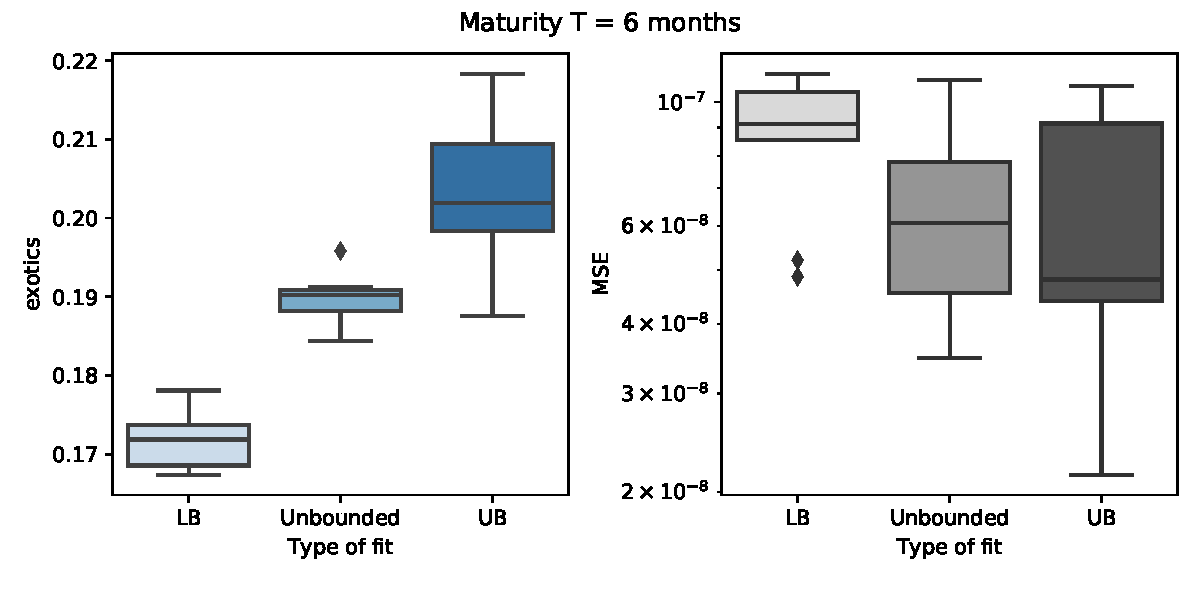
\includegraphics[clip,width=0.75\textwidth]{content/reschap1/Figures/figures_SPX/lookback_bounds_mse.pdf} 
  \caption{Box plots for the Local Stochastic Volatility model~\eqref{eq:LSV_SDE}. Exotic option price quantiles are in blue in the left-hand box-plot groups. The MSE quantiles of market data calibration is in grey, in the right-hand box-plot groups. Each box plot comes from 10 different runs of neural SDE calibration, wherein each run the parameters of the neural SDE are initialised with a different seed. The three box-plots in each group arise respectively from aiming for a lower bound of the illiquid derivative (left), only calibrating to the market and then pricing the illiquid derivative (middle) and aiming for an upper bound of the illiquid derivative (right).}\label{fig:SPX LSV boxplots}
\end{figure}


\subsection{Results from calibrating for LSV neural SDE}
Each calibration is run ten times with different initialisations of the network parameters, with the goal to check the robustness of the exotic option price 
 $\EE^{\QQ(\theta)}[\Psi]$ for each calibrated neural SDE. Each run takes on average 51 minutes on an NVIDIA Tesla V100 SXM2 GPU, meaning that in order to produce each boxplot in Figure~\ref{fig:SPX LSV boxplots} the experiment takes $51 \text{mins} \times 10 = 8.5$ hours. This is repeated to calculate the bounds of the exotic option price. Thus, in total the experiment takes $8.5 \times 3$ hours.
The blue boxplots in Figure~\ref{fig:SPX LSV boxplots} provide different quantiles for the exotic option 
 price $\EE^{\QQ(\theta)}[\Psi]$ and the obtained bounds after running all the experiments $10$ times. 
We make the following observations from calibrating the LSV neural SDE:

\begin{enumerate}[i)]
\item We note that our methods achieve high calibration accuracy to the market data (measured in terms of the MSE) with consistent bounds on the exotic option prices. See MSE in Figure~\ref{fig:SPX LSV boxplots}.
\item The calibration is accurate not only in terms of the MSE on prices (Figure~\ref{fig:SPX LSV boxplots}), but also on the corresponding implied volatility curves, see Figure~\ref{fig:SPX LSV calibration iv} and~\ref{fig:SPX LSV calibration iv error} for calibration to SPX option prices, Figures~\ref{fig:SPX LSV calibration iv lower bound exotic} and~\ref{fig:SPX LSV calibration iv error lower bound exotic} for calibration to SPX option prices minimising the exotic price, Figures~\ref{fig:SPX LSV calibration iv upper bound exotic} and~\ref{fig:SPX LSV calibration iv error upper bound exotic} for calibration to SPX option prices maximising exotic price. The implied volatility curves are calculated using the Python library \texttt{pyvollib}.
\item The LSV neural SDE produces noticeable ranges for prices of illiquid derivatives, see again Figure~\ref{fig:SPX LSV boxplots}.  
\end{enumerate}


\begin{figure}[H]
  \centering 
	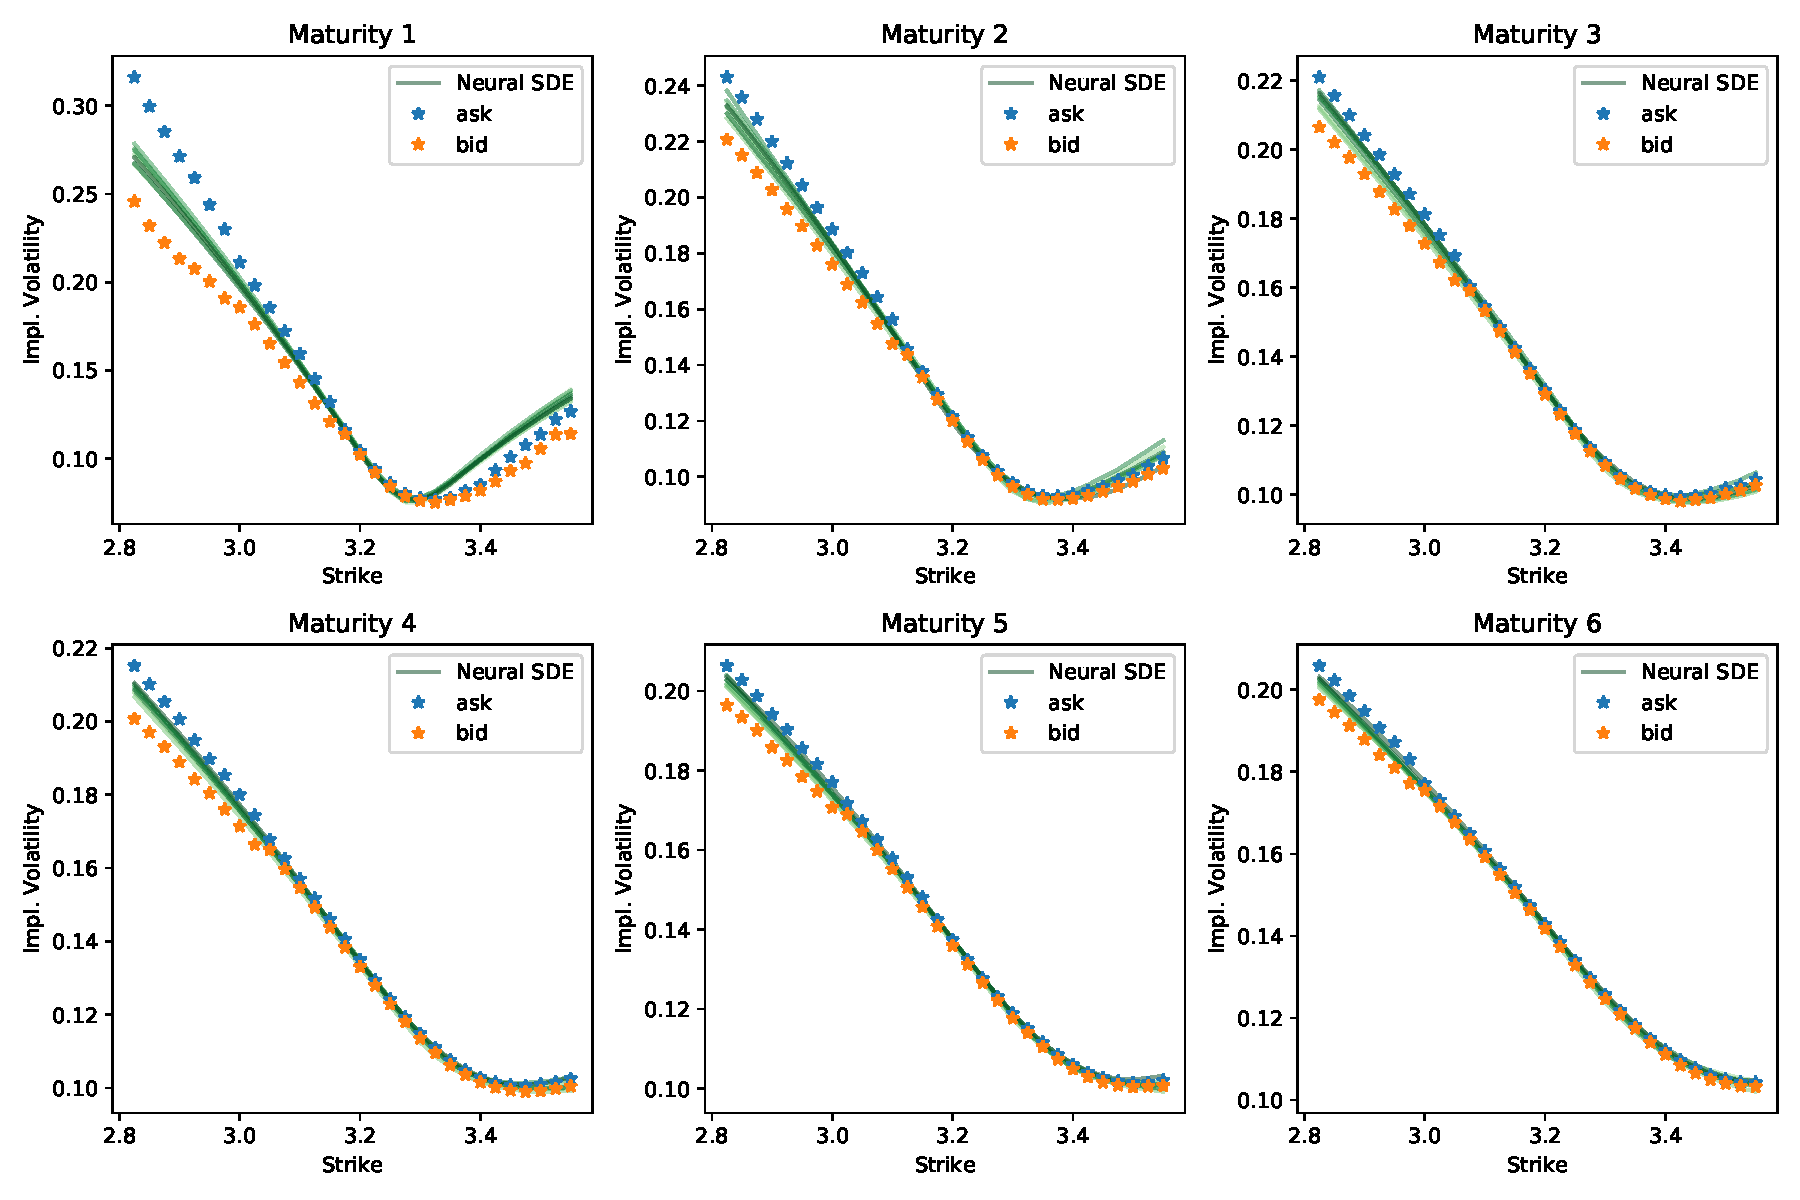
\includegraphics[clip, width=0.7\textwidth]{content/reschap1/Figures/figures_SPX/iv_nsde_unbounded.pdf}
  \caption{Comparing market implied volatility to the model implied volatility for the neural SDE LSV model~\eqref{eq:LSV_SDE} when targeting only the {\em market data}. Strikes from the market data are scaled by a factor of $10^{-3}$. Implied volatility curves of 10 different calibrated neural SDEs are presented in comparison to the market bid-ask spread for different maturities.
}
\label{fig:SPX LSV calibration iv}  
\end{figure}


\begin{figure}[H]
  \centering 
	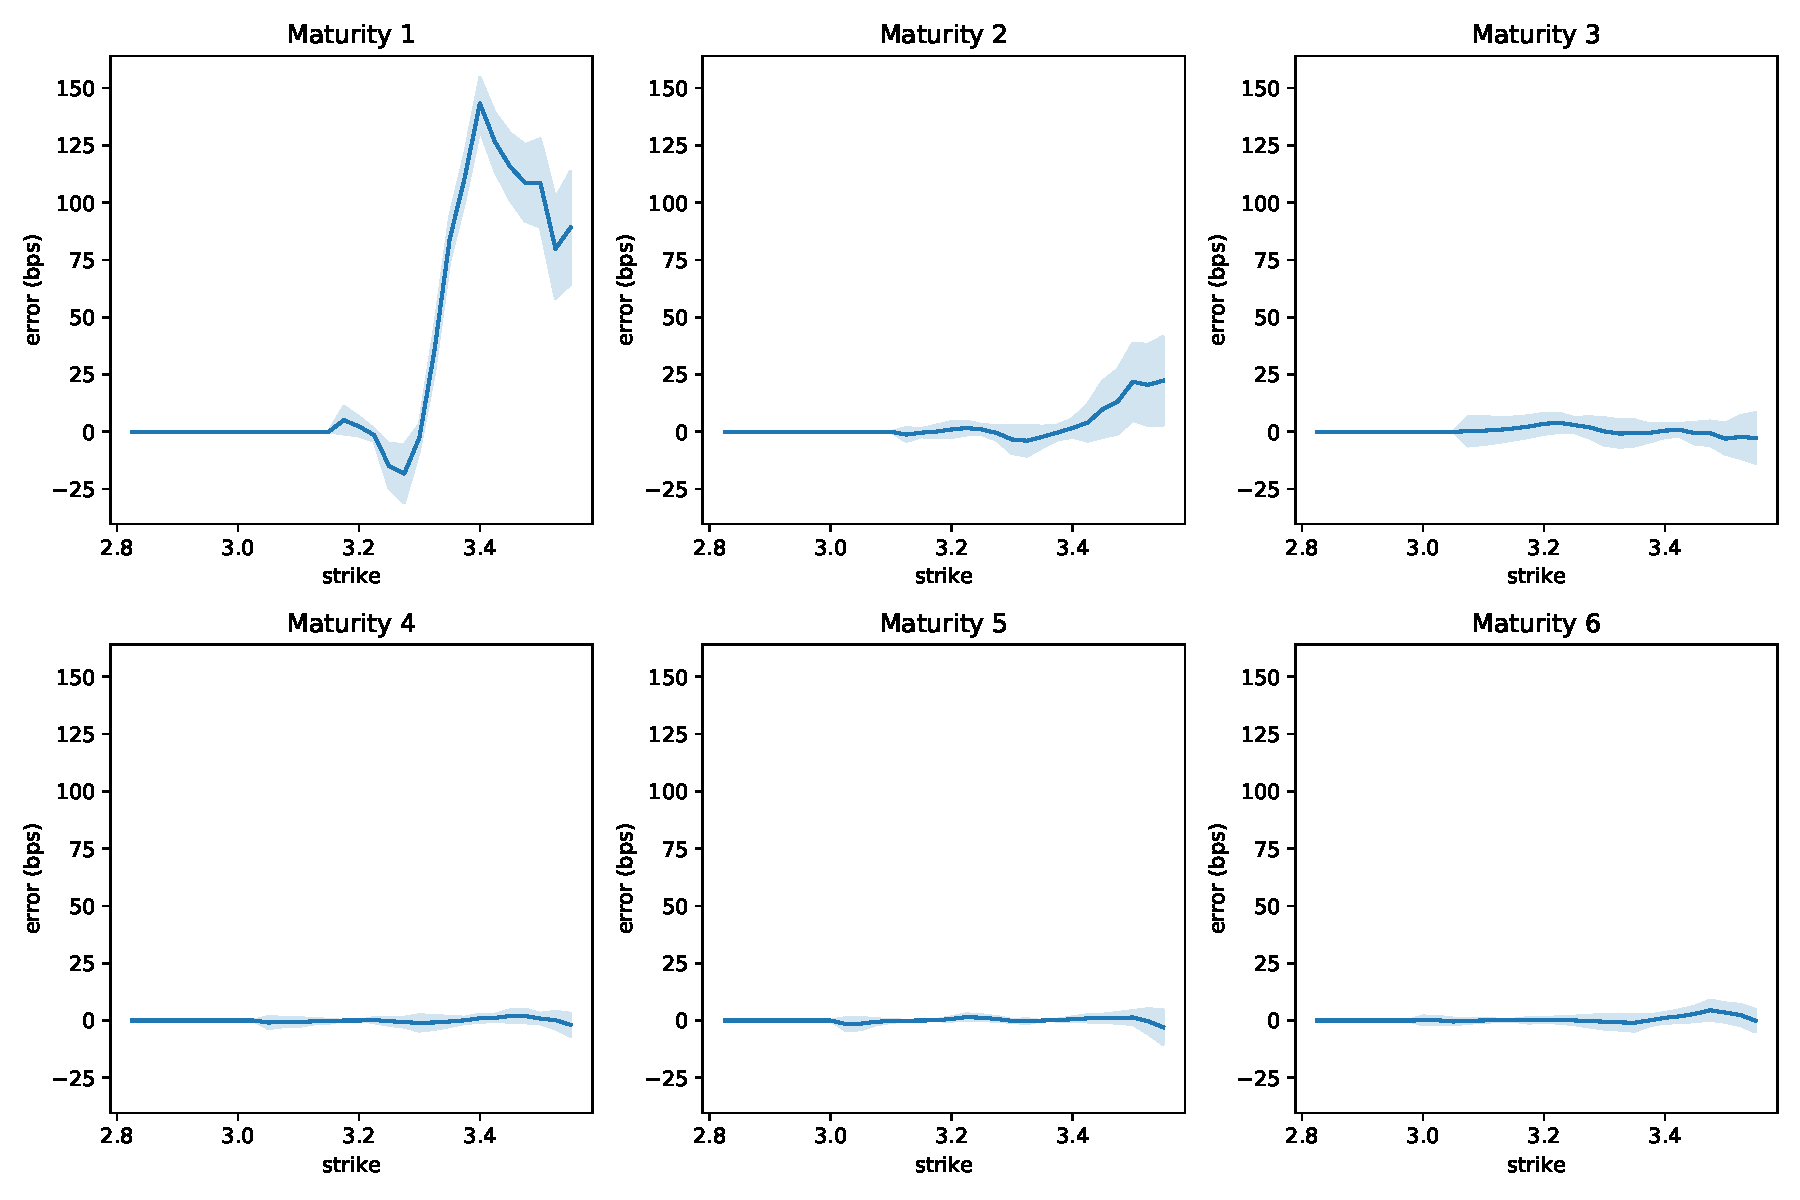
\includegraphics[clip, width=0.66\textwidth]{content/reschap1/Figures/figures_SPX/iv_error_unbounded.pdf}
  \caption{The average error and standard deviation in basis points (bps) of the implied volatility curves from Figure~\ref{fig:SPX LSV calibration iv}. The error is considered to be zero if the implied volatility falls into the bid-ask spread. Strikes from the market data are scaled by a factor of $10^{-3}$.  
}
\label{fig:SPX LSV calibration iv error}  
\end{figure}


\subsection{Hedging strategy evaluation}
We calculate the mean squared error of a learned portfolio hedging strategy of a lookback option at maturity $T=6$ months, given by the empirical variance for a trained set of parameters $\tilde{\theta}\in\Theta\,$:
\[
\Var^{\QQ^N} \left[ \psi\left(X^{\pi,\tilde{\theta}}\right)-\sum_{k=0}^{N_{\text{steps}}-1} \bar{\Hf}\left(t_k, \left\{X_{t_k\wedge t_j}^{\pi,\tilde{\theta}}\right\}_{j=0}^{N_{\text{steps}}}; \xi_{\psi}\right)\Delta \bar S^{\pi,\tilde{\theta}}_{t_{k}} \right] \,.
\]
The histogram in Figure~\ref{fig: SPX eval hedging strategy} is calculated on $N=400\, 000$ different paths and provides the values of $s$ and $s^{\textup{cv}}$, as well as their variances. We can observe a significant reduction in the variance. 
\[
s\defEqual\psi\left(X^{\pi,\tilde{\theta}}\right), \qquad
s^{\textup{cv}}\defEqual \psi\left(X^{\pi,\tilde{\theta}}\right)-\sum_{k=0}^{N_{\text{steps}}-1} \bar{\Hf}\left(t_k, \left\{X_{t_k\wedge t_j}^{\pi,\tilde{\theta}}\right\}_{j=0}^{N_{\text{steps}}}; \xi_{\psi}\right)\Delta \bar S^{\pi,\tilde{\theta}}_{t_{k}},
\]

\begin{figure}[H]\label{fig hedge error}
\centering
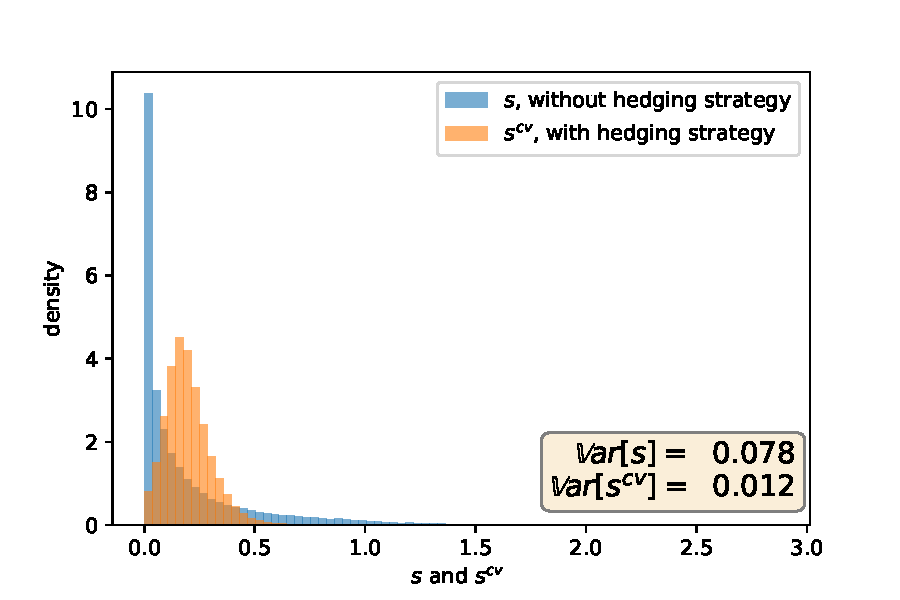
\includegraphics[clip,width=0.6\textwidth]{content/reschap1/Figures/figures_SPX/eval_hedging.pdf}
\caption{Histograms of $s, s^{\textup{cv}}$ with $\Psi$ the lookback option}	
\label{fig: SPX eval hedging strategy}

\end{figure}

\subsection{Joint SPX and VIX calibration}
In this section, we showcase some preliminary results on the calibration of neural SDEs to SPX and VIX data simultaneously. We first describe the setup that was used for modelling. Let $X^\theta=(S^\theta, Y^\theta)$, where $S$ are the traded assets and $Y$ are the components that are not traded. We thus consider the following system of equations
\begin{equation}\label{eq:nsdeSY}
\begin{split}
\D S_t & = S_t \sigma^S(t, S_t, Y_t;\nu)\,\D B^S_t, \quad S_0 = s_0 \,,\\
\D Y_t & = b^Y(t, Y_t; \vartheta^{(b)}) \, \D t +  \sigma^Y(t, Y_t; \vartheta^{(\sigma)})\,\D B^Y_t, \quad Y_0 = y_0\,,\\
\rho \D t &= \D \left\langle B^S, B^ Y\right\rangle_t \,,
\end{split}
\end{equation}
where
$\theta \defEqual  \{\nu, \vartheta^{(b)}, \vartheta^{(\sigma)}, y_0, \rho \},\,\,\rho\in[-1,1],\,y_0\in\RR, 
$
as the set of (multi-dimensional) parameters that we aim to optimise so that 
the model is calibrated to the observed market data. We emphasise that the process $\{Y_t\}_{t\geq 0}$ is not a volatility process per~se, but some general $\RR$-valued stochastic process. It is easy to see that in this model $\{S_t\}_{t\in[0,T]}$ is indeed a (local) martingale. The model is thus free of arbitrage and we can call the measure induced by the model $\QQ(\theta)$ a risk-neutral measure.

\subsubsection{Path-dependent control variate for VIX}\
It quickly becomes apparent that a nested Monte-Carlo procedure is needed for the calculation of prices of VIX derivatives:
\begin{align*}
\EE^{\QQ(\theta)}\left[\phi\left(\VIX_T \right) \right] &= \EE^{\QQ(\theta)}\left[\phi \left( \left\{ \EE\left[ \frac{1}{\Delta} \int_T^{T+\Delta} \sigma^2(s, S_s, Y_s; \nu) \D s \;\middle\vert\; \Ff_T \right] \right\}^\frac{1}{2}\right)\right],
\end{align*}
where $\Delta=1/12$ and $\phi: \RR^+ \to \RR$ is a payoff function. This even further increases the memory requirements of our Algorithm~\ref{alg LSV calibration vanilla} and the reduction of samples becomes even more crucial than in the case of SPX. To this end, we introduce another control variate, which reduces the variance of $\VIX$. Note that the square root prevents us to devise the control variate for $\VIX$ directly, we therefore reduce the variance of $\VIX^2$ instead. Using the path-dependent control variate from \eqref{eq loss cv}, we have:
\begin{align*}
\VIX^2_T &= \EE^{\QQ(\theta)}\left[ \frac{1}{\Delta} \int_T^{T+\Delta} \sigma^2(s, S_s, Y_s; \nu) \, \D s \;\middle\vert\; \Ff_T\right] \\
&= \frac{1}{\Delta} \int_{T}^{T+\Delta} \sigma^{2}(s, S_s, Y_s; \nu) \, \D s -\int_T^{T+\Delta} \Hf \left(s, \left\{\sigma_{s \wedge t}\right\}_{t \in[0, T]} ; \xi^*\right) \D W_{s}
\end{align*}
where $\xi^*$ is given by
\[
\xi^* \in \argmin_\xi \Var^{\QQ^N(\theta)}\left[\frac{1}{\Delta} \int_{T}^{T+\Delta} \sigma^{2}(s, S_s, Y_s; \nu) \, \D s - \int_T^{T+\Delta} \Hf\left(s, \left\{\sigma_{s\wedge t}\right\}_{t\in[0,T]}; \xi\right) \D W_{s} \right]
\]
\subsubsection{Results}
For this part, we use OptionMetrics VIX and SPX data from 20-Dec-2019. We calibrate to OTM European option prices, with the initial price of $s_0=3\,221$ and $\VIX_0=12.51$ for maturities of $1,2,\ldots,6$ months. The neural SDE~\eqref{eq:nsdeSY} is parametrised by neural networks with the same architecture as in Section~\ref{sec:LSV_DL_setting}. We assume a flat forward variance curve and use control variates for both SPX and VIX options as well as VIX futures. As explained above, calibrating to VIX inevitably amounts to nested Monte Carlo simulations. This, together with the fact that the neural SDE is now two-dimensional, contributes to high memory requirements and only allows us to use 2000 outer and 150 inner Monte Carlo samples.

\begin{figure}[H]
\centering
\makebox[\textwidth]{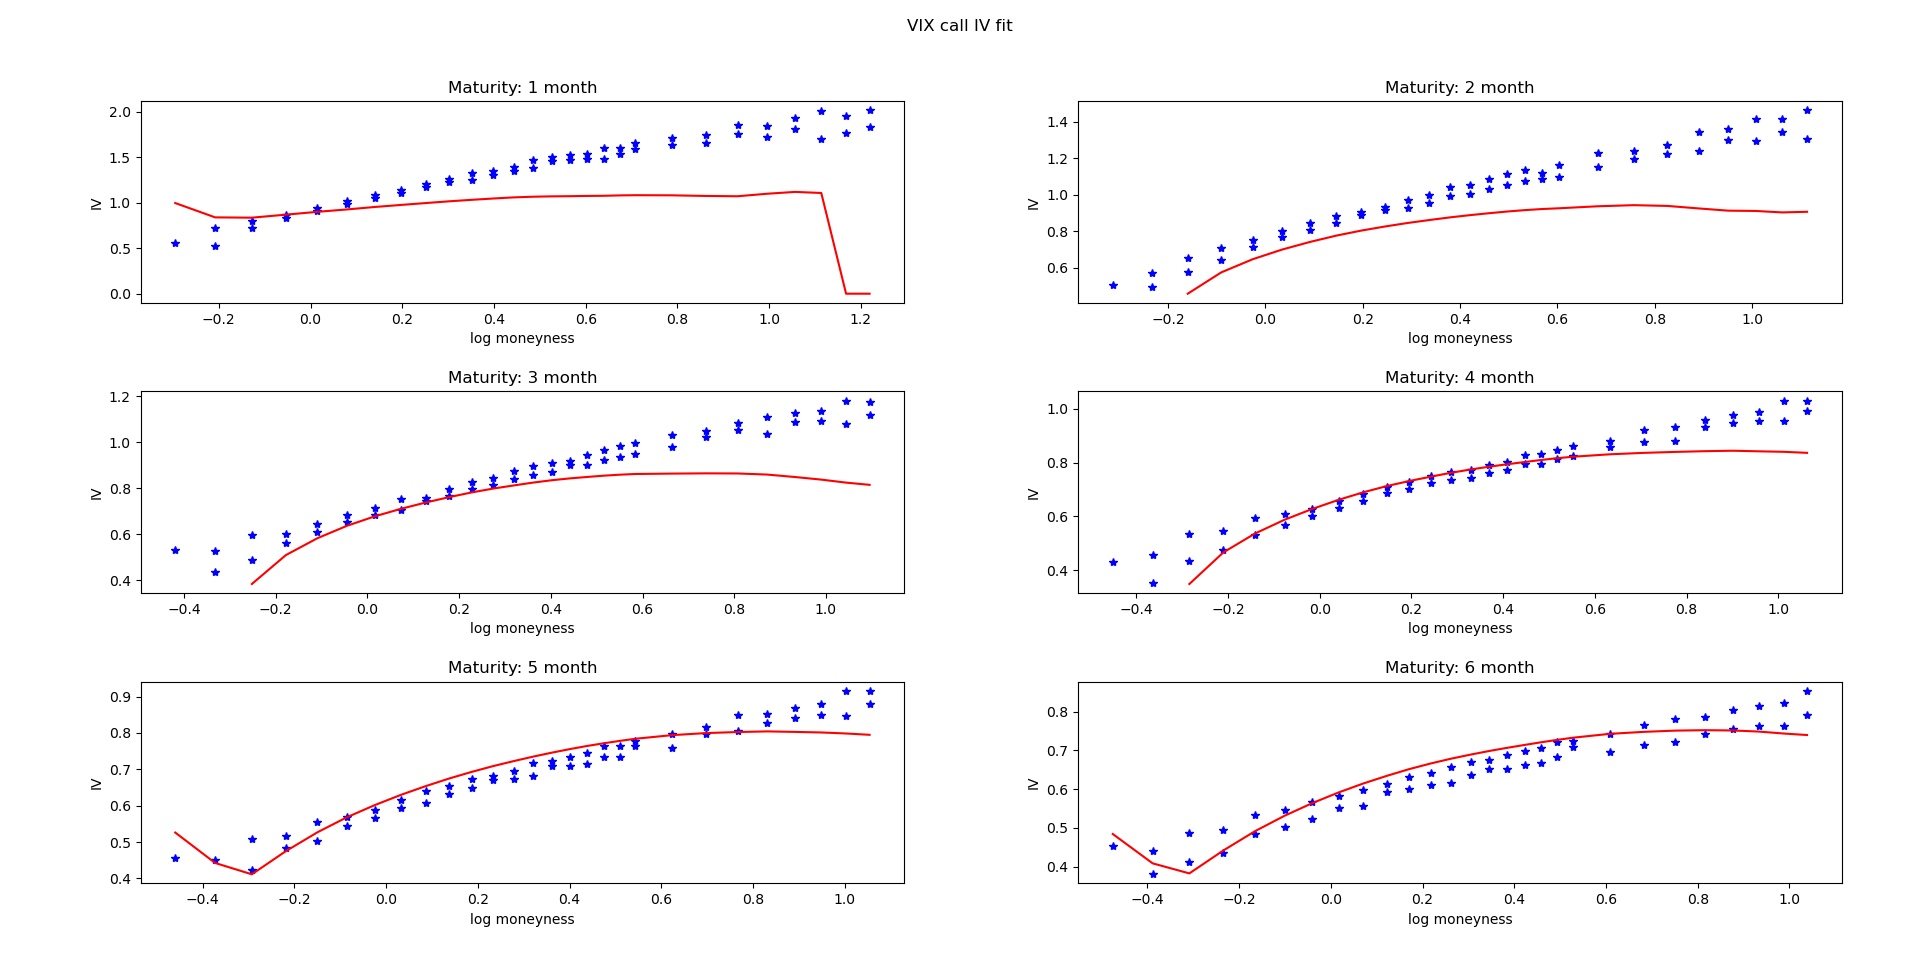
\includegraphics[width=.9\textwidth, height=7.25cm, trim={.5cm .5cm .5cm 2.cm}, clip]{content/reschap1/Figures/Graphics/VIX_call_iv_fit.png}}
\caption{Implied volatility fit of the neural SDE model on VIX Call options on day 20-12-2019.}\label{fig:NSDEvixcall}
\end{figure}


\begin{figure}[H]
\centering
\makebox[\textwidth]{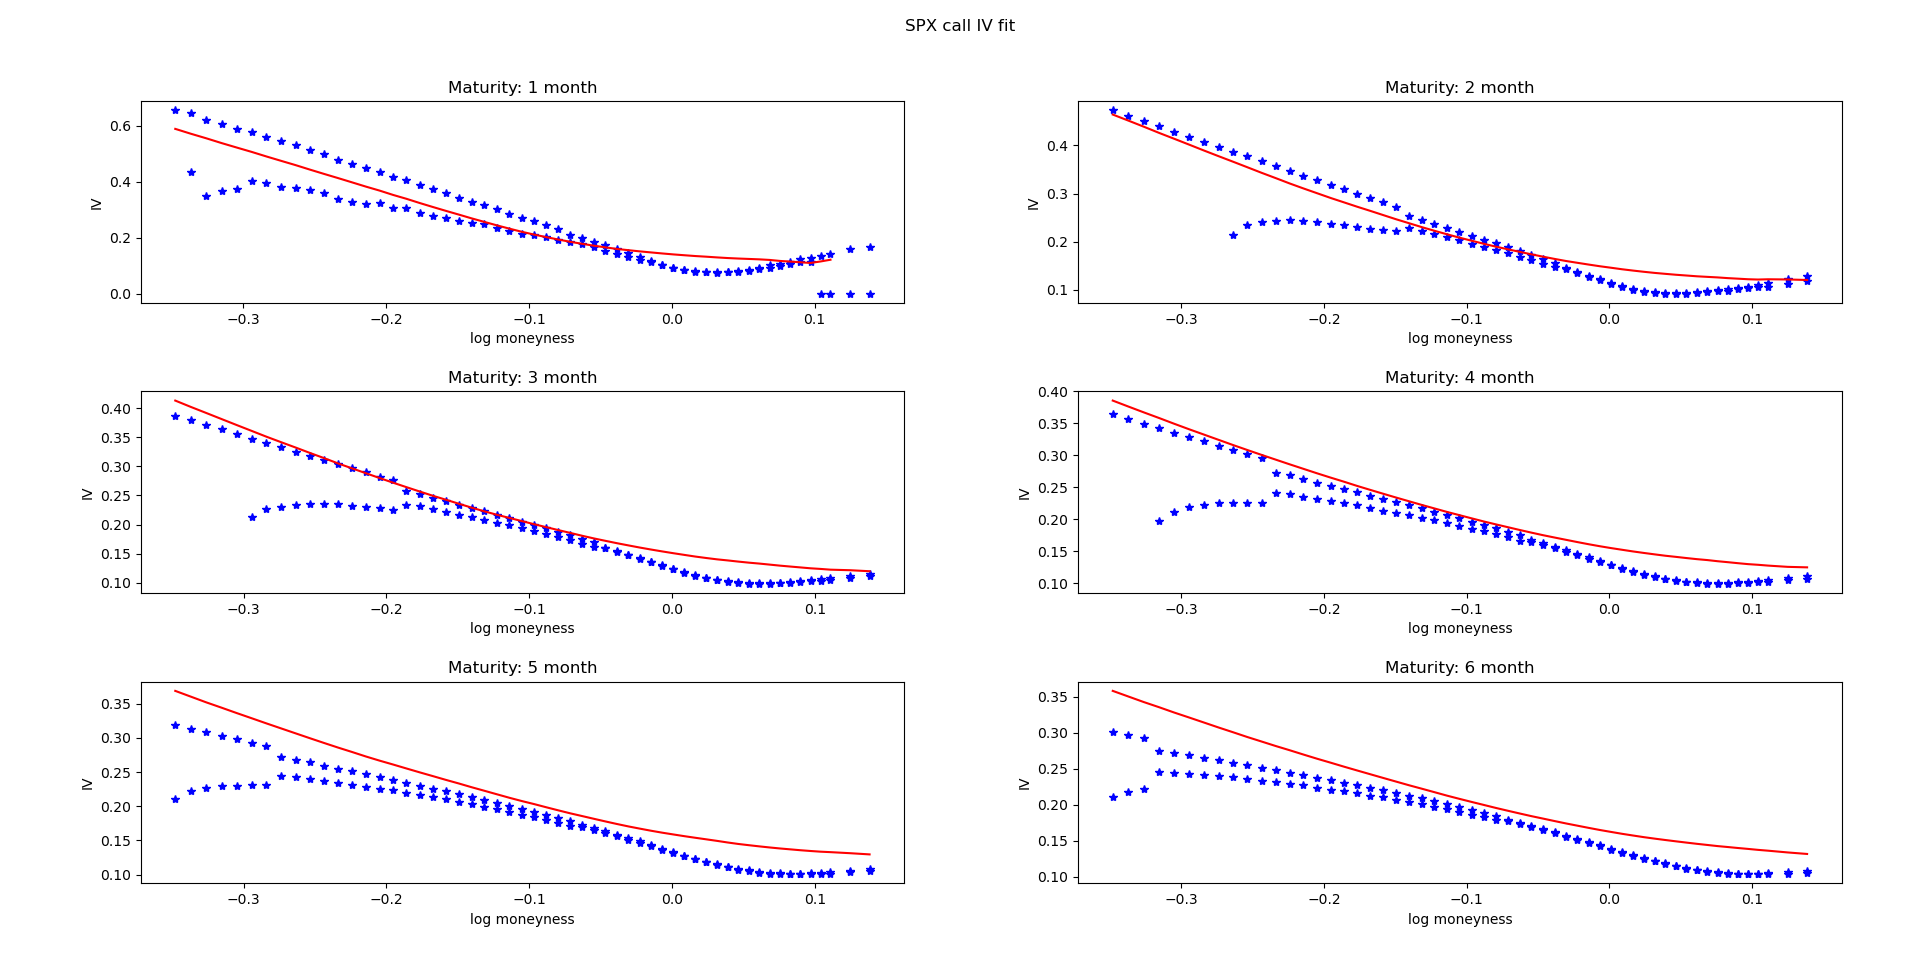
\includegraphics[width=.9\textwidth, height=7.25cm, trim={.5cm .5cm .5cm 2.cm}, clip]{content/reschap1/Figures/Graphics/SPX_call_iv_fit.png}}
\caption{Implied volatility fit of the neural SDE model on SPX Call options on day 20-12-2019.}\label{fig:NSDEspxcall}
\end{figure}

We do not present any detailed error analysis as the poor performance of our joint calibration already becomes apparent from visually comparing implied volatility fits in Figure~\ref{fig:NSDEvixcall} and Figure~\ref{fig:NSDEspxcall} to results from previous sections. We believe the higher errors are a consequence of an inadequate number of samples used (i.e. 20 times fewer samples in the outer loop), due to the scheme being very memory intensive. To be more precise, at the time of writing the cutting-edge GPUs available in retail allow up to only 32Gb of RAM, which presents a major bottleneck for this type of neural SDE model.


